% ============================================================
% PRM393 - OmniCast Mobile project report (English version)
%
% Compile with:
%   xelatex main-en.tex
%   xelatex main-en.tex
% ============================================================
\documentclass[conference,a4paper]{IEEEtran}

% ============================================================
% OmniCast - Shared preamble for IEEEtran conference reports
%   PRN232 (VN / EN) and PRM393 (VN / EN)
%
% Requires: XeLaTeX (MiKTeX / TeX Live)
%   xelatex main-vi.tex && xelatex main-vi.tex
%   xelatex main-en.tex && xelatex main-en.tex
%
% NOTE: IEEEtran already defines its own caption machinery, so the
% `caption` / `subcaption` / `float` packages are intentionally NOT
% loaded here (they clash with IEEEtran). Figure and table labels are
% switched with \renewcommands{\figurename} in the main files.
% ============================================================

% ---------- Language switch ----------
% \bi{Vietnamese text}{English text} picks the right string.
% main-vi.tex calls \omniENfalse (default), main-en.tex calls \omniENtrue.
\newif\ifomniEN
\omniENfalse
\newcommand{\bi}[2]{\ifomniEN#2\else#1\fi}

% ---------- Fonts (Windows system fonts, full Vietnamese coverage) ----------
\usepackage{fontspec}
\setmainfont{Times New Roman}
\setsansfont{Arial}
\setmonofont{Consolas}
\XeTeXlinebreaklocale "vi"
\XeTeXlinebreakskip = 0pt plus 1pt

% ---------- Core packages ----------
\usepackage{amsmath}
\usepackage{amssymb}
\usepackage{booktabs}
\usepackage{multirow}
\usepackage{array}
\usepackage{graphicx}
\usepackage{xcolor}
\usepackage{enumitem}
\usepackage{tikz}
\usepackage{listings}
\usepackage{tabularx}
\usepackage{array}
\usepackage{url}
\usepackage{siunitx}
\usepackage[most]{tcolorbox}
\usepackage{fancyhdr}
\usepackage{lastpage}

% ---------- Page numbering & Running headers/footers ----------
\pagestyle{fancy}
\fancyhf{}
\setlength{\headheight}{14pt}
\renewcommand{\headrulewidth}{0.4pt}
\renewcommand{\footrulewidth}{0.4pt}
\fancyhead[L]{\footnotesize\textsf{\bi{OmniCast --- Báo Cáo Kỹ Thuật Đồ Án PRM393}{OmniCast --- PRM393 Technical Report}}}
\fancyhead[R]{\footnotesize\textsf{\bi{Học Kỳ Fall 2026 (FA26)}{Fall 2026 Semester (FA26)}}}
\fancyfoot[L]{\footnotesize\textsf{\bi{Trường Đại học FPT}{FPT University}}}
\fancyfoot[R]{\footnotesize\textsf{\textbf{\bi{Trang \thepage\ / \pageref{LastPage}}{Page \thepage\ of \pageref{LastPage}}}}}


\usetikzlibrary{positioning,arrows.meta,shapes.geometric,fit,backgrounds,calc,shadows,decorations.pathmorphing}

\usepackage{hyperref}
\pdfstringdefDisableCommands{%
  \ifomniEN\def\bi#1#2{#2}\else\def\bi#1#2{#1}\fi
}
\hypersetup{
  colorlinks=true,
  linkcolor=omniBlue,
  citecolor=omniTeal,
  urlcolor=omniPurple,
  pdftitle={OmniCast Project Report},
  pdfauthor={OmniCast Team},
  pdfsubject={PRN232 / PRM393},
  pdfkeywords={OmniCast, EPG, broadcast, NestJS, Flutter, Next.js}
}

% ---------- OmniCast brand palette ----------
\definecolor{omniBlue}{HTML}{0E7490}
\definecolor{omniDark}{HTML}{0F172A}
\definecolor{omniTeal}{HTML}{0D9488}
\definecolor{omniPurple}{HTML}{7C3AED}
\definecolor{omniAmber}{HTML}{D97706}
\definecolor{omniRose}{HTML}{E11D48}
\definecolor{omniSlate}{HTML}{475569}
\definecolor{omniLight}{HTML}{F1F5F9}
\definecolor{omniBorder}{HTML}{CBD5E1}

% ---------- Typography tweaks ----------
\renewcommand{\familydefault}{\rmdefault}
\setlength{\parindent}{1em}
\setlength{\parskip}{0pt}
\renewcommand{\arraystretch}{1.12}
\setcounter{secnumdepth}{3}

% ---------- Caption / listing labels ----------
% Overridden by the main files so that Vietnamese reports show
% "Hình"/"Bảng" and English reports show "Figure"/"Table".
\newcommand{\figName}{Fig.}
\newcommand{\tabName}{TABLE}
\renewcommand{\figurename}{\figName}
\renewcommand{\tablename}{\tabName}
\providecommand{\lstlistname}{Listing}
\renewcommand{\lstlistname}{Listing}

% ---------- Code listings ----------
\lstdefinestyle{omnicode}{
  backgroundcolor=\color{omniLight},
  basicstyle=\ttfamily\footnotesize,
  keywordstyle=\color{omniBlue}\bfseries,
  stringstyle=\color{omniTeal},
  commentstyle=\color{omniSlate}\itshape,
  numbers=left,
  numberstyle=\tiny\color{omniSlate},
  numbersep=6pt,
  frame=leftline,
  framerule=1.2pt,
  rulecolor=\color{omniBorder},
  breaklines=true,
  breakatwhitespace=true,
  tabsize=2,
  showstringspaces=false,
  columns=fullflexible,
  keepspaces=true,
  xleftmargin=10pt,
  framexleftmargin=8pt,
  captionpos=b
}
\lstset{style=omnicode}

% ---------- TikZ shared styles ----------
\tikzset{
  omniNode/.style={
    draw=omniBorder, fill=white, rounded corners=2pt,
    minimum height=9mm, align=center, font=\footnotesize,
    inner sep=4pt, drop shadow={shadow xshift=0.4pt, shadow yshift=-0.4pt, opacity=0.12}
  },
  omniAccent/.style={omniNode, draw=omniBlue, fill=omniBlue!10, line width=0.8pt},
  omniTealNode/.style={omniNode, draw=omniTeal, fill=omniTeal!10},
  omniAmberNode/.style={omniNode, draw=omniAmber, fill=omniAmber!12},
  omniPurpleNode/.style={omniNode, draw=omniPurple, fill=omniPurple!10},
  omniRoseNode/.style={omniNode, draw=omniRose, fill=omniRose!10},
  omniDarkNode/.style={omniNode, draw=omniDark, fill=omniDark!8},
  omniFlow/.style={-{Latex[length=2.2mm]}, line width=0.7pt, draw=omniSlate},
  omniFlowAccent/.style={-{Latex[length=2.2mm]}, line width=0.9pt, draw=omniBlue},
  omniFlowTeal/.style={-{Latex[length=2.2mm]}, line width=0.9pt, draw=omniTeal},
  omniFlowAmber/.style={-{Latex[length=2.2mm]}, line width=0.9pt, draw=omniAmber},
  omniFlowRose/.style={-{Latex[length=2.2mm]}, line width=0.9pt, draw=omniRose},
  omniLabel/.style={font=\scriptsize\itshape, text=omniSlate}
}

% ---------- Info boxes (tcolorbox) ----------
\newtcolorbox{infobox}[1]{
  enhanced, breakable,
  colback=omniLight!60, colframe=omniBlue,
  fonttitle=\bfseries\small, title={#1},
  boxrule=0.6pt, arc=2pt,
  left=5pt, right=5pt, top=3pt, bottom=3pt
}

\newtcolorbox{warnbox}[1]{
  enhanced, breakable,
  colback=omniAmber!8, colframe=omniAmber,
  fonttitle=\bfseries\small, title={#1},
  boxrule=0.6pt, arc=2pt,
  left=5pt, right=5pt, top=3pt, bottom=3pt
}

\newtcolorbox{keybox}[1]{
  enhanced, breakable,
  colback=omniTeal!7, colframe=omniTeal,
  fonttitle=\bfseries\small, title={#1},
  boxrule=0.6pt, arc=2pt,
  left=5pt, right=5pt, top=3pt, bottom=3pt
}

% ---------- Convenience macros ----------
\newcommand{\omnitag}[1]{\textcolor{omniBlue}{\textbf{#1}}}
\newcommand{\code}[1]{\texttt{\small #1}}
\newcommand{\filepath}[1]{\textcolor{omniSlate}{\textit{\small #1}}}
\newcommand{\vn}[1]{#1}

% ---------- Width fitting ----------
\newcommand{\fitcol}[1]{\resizebox{\columnwidth}{!}{#1}}
\newcommand{\fitfull}[1]{\resizebox{\textwidth}{!}{#1}}

% ---------- Dart language for listings ----------
\lstdefinelanguage{Dart}{
  keywords={abstract, as, assert, async, await, break, case, catch, class, const, continue, default, deferred, do, dynamic, else, enum, export, extends, external, factory, false, final, finally, for, get, if, implements, import, in, is, late, library, new, null, of, on, operator, part, rethrow, return, set, show, static, super, switch, sync, this, throw, true, try, typedef, var, void, while, with, yield},
  morecomment=[l]{//},
  morecomment=[s]{/*}{*/},
  morestring=[b]",
  morestring=[b]'
}

\omniENtrue

% English caption labels
\renewcommand{\figName}{Figure}
\renewcommand{\tabName}{Table}
\renewcommand{\lstlistname}{Listing}

% ============================================================
% OmniCast - Shared TikZ figures (bilingual)
%
% Every visible string uses \bi{Vietnamese}{English} so the same
% source renders correctly in both the VN and the EN report.
%
% Requires the OmniCast preamble (omnicast-preamble-ieee.tex) for
% the colour palette, TikZ styles and the \bi macro.
% ============================================================

% ------------------------------------------------------------
% Figure: Overall layered architecture (PRN232)
% ------------------------------------------------------------
\newcommand{\figArchitecture}{%
\begin{tikzpicture}[scale=0.92, transform shape]
  % --- Presentation layer ---
  \node[omniNode, fill=omniPurple!8, draw=omniPurple] (web) at (0,4.6) {\textbf{Next.js 15 Web Portal}\\App Router $\cdot$ React 19\\Tailwind Cinema Dark};
  \node[omniNode, fill=omniPurple!8, draw=omniPurple] (mob) at (4.0,4.6) {\textbf{Flutter 3.x Mobile}\\BLoC $\cdot$ Dio $\cdot$ Sqflite};

  % --- API layer ---
  \node[omniAccent, minimum width=5.4cm, minimum height=1.5cm] (api) at (2.0,2.5) {\textbf{NestJS 10 REST API}\\19 modules $\cdot$ 140+ endpoints\\JWT + RBAC $\cdot$ Swagger/OpenAPI};
  \node[omniTealNode] (gw) at (2.0,0.9) {\textbf{WebSocket Gateway}\\namespace \texttt{/live}\\Socket.IO $\cdot$ WebRTC signalling};
  \node[omniTealNode] (grpc) at (5.6,0.9) {\textbf{gRPC Client}\\AuditLogger proto};

  % --- Microservice ---
  \node[omniAmberNode] (audit) at (5.6,-0.9) {\textbf{Audit-Logger Microservice}\\NestJS $\cdot$ gRPC server\\Render/own deployment};

  % --- Data layer ---
  \node[omniDarkNode, minimum width=3.0cm] (db) at (0.2,-0.9) {\textbf{PostgreSQL}\\Supabase\\20 Prisma models};
  \node[omniDarkNode] (media) at (2.8,-0.9) {\textbf{MediaMTX}\\WHIP ingest\\HLS / WebRTC out};
  \node[omniDarkNode] (cdn) at (5.0,-0.9) {\textbf{Cloudinary}\\media assets};
  \node[omniDarkNode] (ext) at (7.2,-0.9) {\textbf{External APIs}\\OpenAI $\cdot$ TMDB\\YouTube/Twitch/RSS};

  % --- Flows ---
  \draw[omniFlowAccent] (web) -- (api);
  \draw[omniFlowAccent] (mob) -- (api);
  \draw[omniFlow] (api) -- (gw);
  \draw[omniFlow] (api) -- (grpc);
  \draw[omniFlowTeal] (grpc) -- (audit);
  \draw[omniFlow] (api) -- (db);
  \draw[omniFlow] (api) -- (media);
  \draw[omniFlow] (api) -- (cdn);
  \draw[omniFlowAmber] (api) -- (ext);
  \draw[omniFlow] (media) -- (mob);
  \draw[omniFlow] (media) -- (web);

  % --- Layer annotations ---
  \node[omniLabel, anchor=west] at (-1.85,4.6) {\bi{\textbf{Tầng}}{\textbf{Presentation}}};
  \node[omniLabel, anchor=west] at (-1.85,2.5) {\bi{\textbf{API}}{\textbf{API}}};
  \node[omniLabel, anchor=west] at (-1.85,0.9) {\bi{\textbf{Real-time}}{\textbf{Real-time}}};
  \node[omniLabel, anchor=west] at (-1.85,-0.9) {\bi{\textbf{Dữ liệu}}{\textbf{Data}}};
\end{tikzpicture}%
}

% ------------------------------------------------------------
% Figure: EPG anti-conflict scheduling timeline
% ------------------------------------------------------------
\newcommand{\figScheduleConflict}{%
\begin{tikzpicture}[x=0.95cm, y=0.75cm]
  % Existing event on the channel
  \filldraw[fill=omniBlue!22, draw=omniBlue, line width=0.8pt]
    (1.0,1.6) rectangle (5.2,2.3);
  \node at (3.1,1.95) {\footnotesize \bi{\textbf{Sự kiện đã có}}{\textbf{Existing event}} (14:00--15:00)};

  % Candidate event - overlapping head
  \filldraw[fill=omniRose!20, draw=omniRose, line width=0.8pt]
    (0.4,0.45) rectangle (4.2,1.15);
  \node at (2.3,0.8) {\footnotesize \bi{\textbf{Lịch mới}}{\textbf{New schedule}} (13:30--14:30)};
  \node[omniRose, font=\scriptsize\bfseries] at (2.3,0.15) {\bi{giao thoa đầu $\rightarrow$ 409}{head overlap $\rightarrow$ 409}};

  % Candidate event - overlapping tail
  \filldraw[fill=omniRose!20, draw=omniRose, line width=0.8pt]
    (4.0,2.85) rectangle (7.2,3.55);
  \node at (5.6,3.2) {\footnotesize \bi{\textbf{Lịch mới}}{\textbf{New schedule}} (14:30--15:30)};
  \node[omniRose, font=\scriptsize\bfseries] at (5.6,2.6) {\bi{giao thoa đuôi $\rightarrow$ 409}{tail overlap $\rightarrow$ 409}};

  % Candidate event - fully contained
  \filldraw[fill=omniRose!20, draw=omniRose, line width=0.8pt]
    (0.9,3.4) rectangle (5.6,4.1);
  \node at (3.25,3.75) {\footnotesize \bi{\textbf{Lịch mới}}{\textbf{New schedule}} (13:00--16:00)};
  \node[omniRose, font=\scriptsize\bfseries] at (3.25,3.15) {\bi{bao trùm toàn bộ $\rightarrow$ 409}{fully contained $\rightarrow$ 409}};

  % Non-overlapping on another channel
  \filldraw[fill=omniTeal!20, draw=omniTeal, line width=0.8pt]
    (6.0,0.45) rectangle (9.4,1.15);
  \node at (7.7,0.8) {\footnotesize \bi{\textbf{Kênh khác}}{\textbf{Other channel}} (14:00--15:00)};
  \node[omniTeal, font=\scriptsize\bfseries] at (7.7,0.15) {\bi{cho phép $\rightarrow$ 201}{allowed $\rightarrow$ 201}};

  % Time axis
  \draw[-{Latex[length=2mm]}, line width=0.6pt] (0.2,0) -- (9.8,0);
  \foreach \x/\lab in {1.0/13:00,2.6/14:00,4.2/15:00,5.8/16:00,7.4/17:00,9.0/18:00}{
    \draw (\x,0) -- (\x,0.12);
    \node[font=\scriptsize, below=2pt] at (\x,0) {\lab};
  }
\end{tikzpicture}%
}

% ------------------------------------------------------------
% Figure: AI Curator pipeline (consolidated single call + fallback)
% ------------------------------------------------------------
\newcommand{\figAiPipeline}{%
\begin{tikzpicture}[node distance=0.9cm and 1.3cm]
  \node[omniNode] (input) {\bi{\textbf{Đầu vào}}{\textbf{Input}}\\title + description\\category + tags};
  \node[omniAccent, right=of input] (norm) {\bi{\textbf{Chuẩn hoá}}{\textbf{Normalise}}\\\texttt{CuratorProgramInput}};
  \node[omniAmberNode, right=of norm] (branch) {\bi{\textbf{Phân nhánh}}{\textbf{Branch}}\\\bi{có \texttt{OPENAI\_API\_KEY}?}{has \texttt{OPENAI\_API\_KEY}?}};

  \node[omniTealNode, above right=0.4cm and 1.6cm of branch] (prompt) {\textbf{buildConsolidatedPrompt}\\temperature 0.3 $\cdot$ top\_p 0.95};
  \node[omniTealNode, right=of prompt] (call) {\bi{\textbf{Gọi OpenAI}}{\textbf{Call OpenAI}}\\gpt-4o $\cdot$ retry + backoff};
  \node[omniDarkNode, right=of call] (valid) {\bi{\textbf{Kiểm tra schema}}{\textbf{Schema check}}\\Zod validate};

  \node[omniRoseNode, below right=0.4cm and 1.6cm of branch] (fallback) {\bi{\textbf{Heuristic fallback}}{\textbf{Heuristic fallback}}\\\texttt{sentiment / compliance / editorial}};
  \node[omniPurpleNode, right=of fallback] (conf) {\bi{\textbf{Tính confidence}}{\textbf{Compute confidence}}\\heuristic $\cdot$ clamp 0..1};

  \node[omniAccent, right=of valid, minimum width=2.4cm] (report) {\textbf{AiCuratorReport}\\\bi{\texttt{lưu trong PostgreSQL}}{\texttt{stored in PostgreSQL}}};
  \node[omniNode, below=of report] (stamp) {\bi{\textbf{Dấu vết}}{\textbf{Provenance}}\\\texttt{promptVersion} $\cdot$ \texttt{aiModelVersion}\\\texttt{openaiCallMs} $\cdot$ \texttt{openaiRetries}};

  \draw[omniFlowAccent] (input) -- (norm);
  \draw[omniFlowAccent] (norm) -- (branch);
  \draw[omniFlowTeal] (branch) -- node[above, font=\scriptsize] {\bi{có}{yes}} (prompt);
  \draw[omniFlowTeal] (prompt) -- (call);
  \draw[omniFlowTeal] (call) -- (valid);
  \draw[omniFlowRose] (branch) -- node[below, font=\scriptsize] {\bi{không}{no}} (fallback);
  \draw[omniFlowRose] (fallback) -- (conf);
  \draw[omniFlowTeal] (valid) -- (report);
  \draw[omniFlowRose] (conf) -- (report);
  \draw[omniFlow] (report) -- (stamp);
  \draw[omniFlowRose, dashed] (valid) to[out=200,in=20] node[font=\scriptsize, text=omniRose] {validate fail} (fallback);
\end{tikzpicture}%
}

% ------------------------------------------------------------
% Figure: Mobile BLoC layered architecture (PRM393)
% ------------------------------------------------------------
\newcommand{\figMobileArchitecture}{%
\begin{tikzpicture}[scale=0.95, transform shape]
  \begin{scope}[local bounding box=pres]
    \node[omniPurpleNode, minimum width=5.0cm, minimum height=1.4cm] (pres) at (0,3.4) {\bi{\textbf{Tầng Presentation}}{\textbf{Presentation layer}}\\31 screens $\cdot$ 22 widgets\\GoRouter navigation};
  \end{scope}

  \begin{scope}[local bounding box=logic]
    \node[omniAccent, minimum width=5.0cm, minimum height=1.4cm] (logic) at (0,1.5) {\bi{\textbf{Tầng Logic (BLoC)}}{\textbf{Logic layer (BLoC)}}\\12 BLoC/Cubit\\events $\rightarrow$ states};
  \end{scope}

  \begin{scope}[local bounding box=data]
    \node[omniTealNode, minimum width=5.0cm, minimum height=1.4cm] (data) at (0,-0.4) {\bi{\textbf{Tầng Data}}{\textbf{Data layer}}\\10 repositories $\cdot$ 10 models\\Dio client $\cdot$ AuthInterceptor};
  \end{scope}

  \begin{scope}[local bounding box=core]
    \node[omniDarkNode, minimum width=5.0cm, minimum height=1.4cm] (core) at (0,-2.3) {\bi{\textbf{Tầng Core}}{\textbf{Core layer}}\\DI (get\_it) $\cdot$ theme $\cdot$ i18n\\constants $\cdot$ utils $\cdot$ services};
  \end{scope}

  \node[omniAmberNode, right=1.4cm of data] (local) {\bi{\textbf{Lưu trữ cục bộ}}{\textbf{Local Storage}}\\\texttt{omnicast\_local.db}\\Sqflite offline-first};
  \node[omniRoseNode, right=1.4cm of core] (remote) {\bi{\textbf{Từ xa}}{\textbf{Remote}}\\REST API (NestJS)\\FCM push $\cdot$ Supabase Realtime};

  \draw[omniFlowAccent] (pres) -- node[right, font=\scriptsize] {dispatch} (logic);
  \draw[omniFlowAccent] (logic) -- node[right, font=\scriptsize] {\bi{gọi}{calls}} (data);
  \draw[omniFlowTeal] (data) -- (local);
  \draw[omniFlowRose] (data) -- (remote);
  \draw[omniFlow, dashed] (core) -- (data);
\end{tikzpicture}%
}

% ------------------------------------------------------------
% Figure: Offline-first watchlist sync flow
% ------------------------------------------------------------
\newcommand{\figOfflineSync}{%
\begin{tikzpicture}[node distance=1.0cm and 1.4cm]
  \node[omniNode] (ui) {\textbf{WatchlistScreen}\\SaveToWatchlistButton};
  \node[omniAccent, right=of ui] (bloc) {\textbf{WatchlistBloc}\\\texttt{AddToWatchlist}\\\texttt{LoadWatchlist}};
  \node[omniTealNode, right=of bloc] (repo) {\textbf{WatchlistRepository}};

  \node[omniAmberNode, below=of repo] (sqlite) {\textbf{SQLite}\\\texttt{omnicast\_local.db}\\\texttt{WatchlistCache}};
  \node[omniRoseNode, right=of sqlite] (api) {\textbf{REST}\\\texttt{GET/POST /me/watchlist}};
  \node[omniDarkNode, right=of api] (notif) {\bi{\textbf{Thông báo cục bộ}}{\textbf{Local notification}}\\\bi{đặt lịch trước 15 phút}{schedule 15 min ahead}};

  \draw[omniFlowAccent] (ui) -- (bloc);
  \draw[omniFlowAccent] (bloc) -- (repo);
  \draw[omniFlowTeal] (repo) -- (sqlite);
  \draw[omniFlowRose] (repo) -- (api);
  \draw[omniFlow] (sqlite) -- (notif);
  \draw[omniFlowRose, dashed] (api) to[out=0,in=180] node[above, font=\scriptsize] {\bi{đồng bộ khi online}{sync online}} (sqlite);
  \draw[omniFlowAmber, dashed] (sqlite) to[out=200,in=20] node[below, font=\scriptsize, text=omniAmber] {\bi{đọc offline khi mất mạng}{read offline when offline}} (ui);
\end{tikzpicture}%
}

% ------------------------------------------------------------
% Figure: CI/CD pipeline
% ------------------------------------------------------------
\newcommand{\figCicd}{%
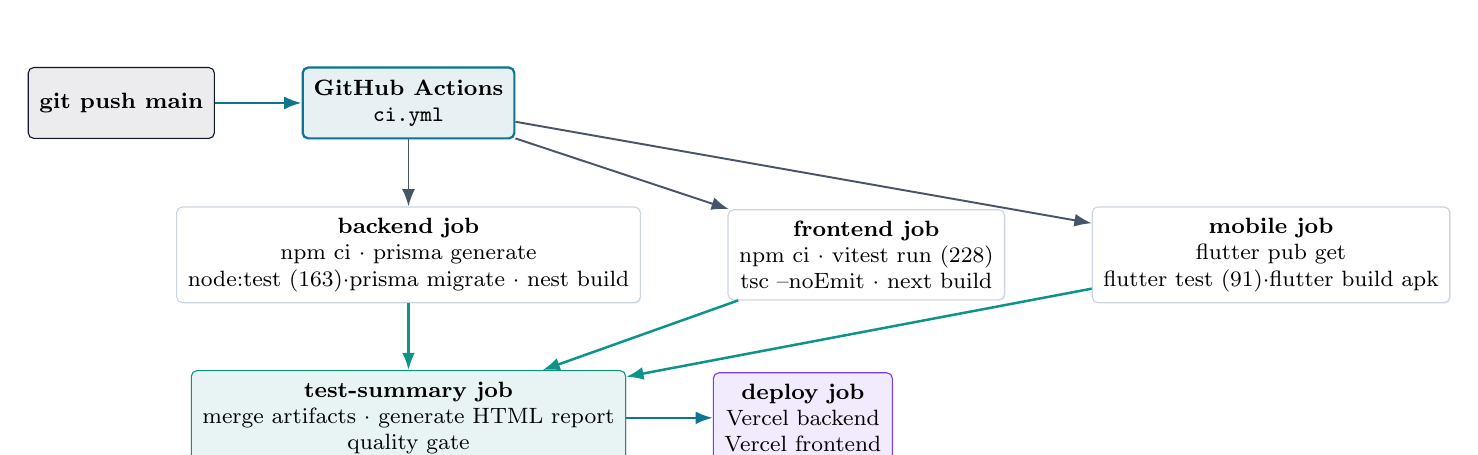
\begin{tikzpicture}[node distance=0.85cm and 1.1cm]
  \node[omniDarkNode] (push) {\textbf{git push main}};
  \node[omniAccent, right=of push] (gha) {\textbf{GitHub Actions}\\\texttt{ci.yml}};

  \node[omniNode, below=of gha] (be) {\bi{\textbf{backend job}}{\textbf{backend job}}\\npm ci $\cdot$ prisma generate\\node:test (163)$\cdot$prisma migrate $\cdot$ nest build};
  \node[omniNode, right=of be] (fe) {\bi{\textbf{frontend job}}{\textbf{frontend job}}\\npm ci $\cdot$ vitest run (228)\\tsc --noEmit $\cdot$ next build};
  \node[omniNode, right=of fe] (mob) {\bi{\textbf{mobile job}}{\textbf{mobile job}}\\flutter pub get\\flutter test (91)$\cdot$flutter build apk};

  \node[omniTealNode, below=of be] (sum) {\bi{\textbf{test-summary job}}{\textbf{test-summary job}}\\merge artifacts $\cdot$ generate HTML report\\quality gate};
  \node[omniPurpleNode, right=of sum] (dep) {\bi{\textbf{deploy job}}{\textbf{deploy job}}\\Vercel backend\\Vercel frontend};

  \draw[omniFlowAccent] (push) -- (gha);
  \draw[omniFlow] (gha) -- (be);
  \draw[omniFlow] (gha) -- (fe);
  \draw[omniFlow] (gha) -- (mob);
  \draw[omniFlowTeal] (be) -- (sum);
  \draw[omniFlowTeal] (fe) -- (sum);
  \draw[omniFlowTeal] (mob) -- (sum);
  \draw[omniFlowAccent] (sum) -- (dep);
\end{tikzpicture}%
}

% ------------------------------------------------------------
% Figure: JWT authentication & RBAC flow
% ------------------------------------------------------------
\newcommand{\figAuthFlow}{%
\begin{tikzpicture}[node distance=0.9cm and 1.2cm]
  \node[omniNode] (client) {\bi{\textbf{Client}}{\textbf{Client}}\\\bi{Web hoặc Mobile}{Web or Mobile}};
  \node[omniAccent, right=of client] (auth) {\textbf{AuthController}\\\texttt{/api/v1/auth/login}};
  \node[omniTealNode, right=of auth] (svc) {\textbf{AuthService}\\bcrypt verify\\deactivated check};
  \node[omniDarkNode, right=of svc] (db) {\textbf{PostgreSQL}\\\texttt{User} + \texttt{RefreshToken}};

  \node[omniPurpleNode, below=of svc] (tok) {\bi{\textbf{Cấp token}}{\textbf{Issue tokens}}\\\texttt{access} 60 min\\\texttt{refresh} 90 days (rotated)};
  \node[omniAmberNode, right=of tok] (guard) {\bi{\textbf{RBAC Guards}}{\textbf{RBAC Guards}}\\\texttt{JwtAuthGuard}\\\texttt{RolesGuard}};
  \node[omniRoseNode, right=of guard] (api) {\bi{\textbf{Endpoint có kiểm tra quyền}}{\textbf{Role-guarded endpoint}}\\\texttt{@Roles(1,2,3)}};

  \draw[omniFlowAccent] (client) -- (auth);
  \draw[omniFlowAccent] (auth) -- (svc);
  \draw[omniFlow] (svc) -- (db);
  \draw[omniFlowTeal] (svc) -- (tok);
  \draw[omniFlowTeal] (tok) -- (guard);
  \draw[omniFlowRose] (guard) -- (api);
  \draw[omniFlow, dashed] (client) to[out=0,in=180] node[above, font=\scriptsize] {Bearer token} (guard);
\end{tikzpicture}%
}

% ------------------------------------------------------------
% Figure: Ingest pipeline (external sources -> normalised events)
% ------------------------------------------------------------
\newcommand{\figIngest}{%
\begin{tikzpicture}[node distance=0.85cm and 1.2cm]
  \node[omniAmberNode] (yt) {\textbf{YouTube}\\Data API v3};
  \node[omniAmberNode, below=of yt] (tw) {\textbf{Twitch}\\Helix API};
  \node[omniAmberNode, below=of tw] (rss) {\textbf{RSS}\\Feed parser};

  \node[omniAccent, right=of yt] (cron) {\bi{\textbf{Bộ lập lịch}}{\textbf{Scheduler}}\\\texttt{@Cron}\\\bi{15'/30' phút}{15'/30' minutes}};
  \node[omniTealNode, right=of cron] (norm) {\bi{\textbf{Chuẩn hoá}}{\textbf{Normalise}}\\\texttt{NormalizedLiveEvent}\\duration in seconds};
  \node[omniDarkNode, right=of norm] (db) {\textbf{LiveEvent}\\\bi{upsert theo kênh}{upsert per channel}};
  \node[omniRoseNode, right=of db] (fill) {\bi{\textbf{Điền lịch trống}}{\textbf{EPG filler}}\\24/7 grid};

  \draw[omniFlowAmber] (yt) -- (cron);
  \draw[omniFlowAmber] (tw) -- (cron);
  \draw[omniFlowAmber] (rss) -- (cron);
  \draw[omniFlowAccent] (cron) -- (norm);
  \draw[omniFlowTeal] (norm) -- (db);
  \draw[omniFlowRose] (db) -- (fill);
\end{tikzpicture}%
}


\begin{document}

% ============================================================
% PRM393 - Academic Cover Page (Trang Bìa Đồ Án FPT University)
% ============================================================
\onecolumn
\thispagestyle{empty}

\begin{tikzpicture}[remember picture, overlay]
  % Khung viền đôi trang trọng
  \draw[line width=2pt, color=omniDark] 
    ($(current page.north west) + (20mm,-20mm)$) 
    rectangle 
    ($(current page.south east) + (-15mm,20mm)$);
  \draw[line width=0.8pt, color=omniBlue] 
    ($(current page.north west) + (21.5mm,-21.5mm)$) 
    rectangle 
    ($(current page.south east) + (-16.5mm,21.5mm)$);
  \fill[omniBlue] ($(current page.north west) + (21.5mm,-21.5mm)$) circle (2.5pt);
  \fill[omniBlue] ($(current page.north east) + (-16.5mm,-21.5mm)$) circle (2.5pt);
  \fill[omniBlue] ($(current page.south west) + (21.5mm,21.5mm)$) circle (2.5pt);
  \fill[omniBlue] ($(current page.south east) + (-16.5mm,21.5mm)$) circle (2.5pt);
\end{tikzpicture}

\begin{center}
  \vspace*{-6mm}
  {\bfseries\large\bi{BỘ GIÁO DỤC VÀ ĐÀO TẠO}{MINISTRY OF EDUCATION AND TRAINING}}\\[2mm]
  {\bfseries\Large\bi{TRƯỜNG ĐẠI HỌC FPT}{FPT UNIVERSITY}}\\[1.5mm]
  {\small\bi{KHOA CÔNG NGHỆ THÔNG TIN --- BỘ MÔN KỸ THUẬT PHẦN MỀM}{FACULTY OF INFORMATION TECHNOLOGY --- SOFTWARE ENGINEERING}}\\[8mm]

  % Huy hiệu nhận diện ứng dụng OmniCast Mobile
  \begin{tikzpicture}
    \node[draw=omniBlue, fill=omniLight, rounded corners=6pt, line width=1.2pt, inner sep=6pt] {
      \textbf{\large\textcolor{omniDark}{OMNI}\textcolor{omniBlue}{CAST MOBILE}}
      \quad\textcolor{omniSlate}{\footnotesize$\vert$}\quad
      \textcolor{omniDark}{\footnotesize\bfseries\bi{ỨNG DỤNG DI ĐỘNG NATIVE FLUTTER}{NATIVE FLUTTER CLIENT}}
    };
  \end{tikzpicture}
  \vspace{8mm}

  {\Large\bfseries\bi{BÁO CÁO NGHIỆM THU ĐỒ ÁN HỌC PHẦN}{FINAL PROJECT DELIVERABLE REPORT}}\\[3mm]
  {\large\bfseries\bi{HỌC PHẦN: PRM393 --- PHÁT TRIỂN ỨNG DỤNG DI ĐỘNG}{COURSE: PRM393 --- MOBILE APPLICATIONS DEVELOPMENT}}\\[8mm]

  {\color{omniBlue}\rule{0.85\linewidth}{1.6pt}}\\[5mm]
  {\LARGE\bfseries\bi{ỨNG DỤNG DI ĐỘNG PHÁT SÓNG VÀ}{OMNICAST MOBILE: ENTERPRISE BROADCAST}}\\[2.5mm]
  {\LARGE\bfseries\bi{TRUYỀN HÌNH TRỰC TUYẾN OMNICAST MOBILE}{\& INTERACTIVE STREAMING CLIENT}}\\[3mm]
  {\large\bfseries\textcolor{omniBlue}{Cross-Platform Broadcast \& Interactive Multimedia Streaming Client}}\\[3mm]
  {\normalsize\itshape\bi{Kiến trúc Clean Architecture 4 tầng, Quản lý trạng thái BLoC, Bộ nhớ đệm SQLite ngoại tuyến (Offline-First) và Trình phát OmniPlayer độ trễ thấp WebRTC/HLS}{4-Tier Clean Architecture, BLoC State Management, Offline-First SQLite Cache, and Ultra-Low Latency WebRTC/HLS OmniPlayer}}\\[4mm]
  {\color{omniBlue}\rule{0.85\linewidth}{1.6pt}}\\[8mm]

  \begin{tcolorbox}[
    colback=white, colframe=omniBorder, boxrule=0.8pt, arc=3pt,
    width=0.88\linewidth, left=8mm, right=8mm, top=4mm, bottom=4mm
  ]
  \renewcommand{\arraystretch}{1.3}
  \begin{tabular}{ll}
    \textbf{\bi{Giảng viên hướng dẫn:}{Course Instructor:}} & \bi{Bộ môn Kỹ thuật Phần mềm (SE)}{Department of Software Engineering} \\
    \textbf{\bi{Học kỳ thực hiện:}{Academic Semester:}}     & Fall 2026 (FA26) \\
    \textbf{\bi{Nhóm tác giả:}{Author Team:}}              & OmniCast Engineering Group \\
    \textbf{\bi{Kho mã nguồn (GitHub):}{GitHub Repository:}} & \url{https://github.com/TomOutfit/OmniCast_PRN232-PRM393_Project_Fa26Semester} \\
    \textbf{\bi{Bản phát hành APK:}{Mobile Release (APK):}}  & \url{https://github.com/TomOutfit/OmniCast_PRN232-PRM393_Project_Fa26Semester/releases/tag/v1.2.0} \\
    \textbf{\bi{Quy mô \& Kiểm định:}{Scale \& Verification:}} & \textbf{\bi{53.922 dòng mã Dart $\vert$ 91/91 Tests PASS (100\%)}{53,922 Dart LOC $\vert$ 91/91 Tests PASS (100\%)}} \\
  \end{tabular}
  \end{tcolorbox}

  \vfill
  {\bfseries\bi{HÀ NỘI / TP. HỒ CHÍ MINH --- THÁNG 10 NĂM 2026}{VIETNAM --- OCTOBER 2026}}\\[2mm]
\end{center}

\clearpage
\twocolumn


\pagenumbering{arabic}
\setcounter{page}{1}
\pagestyle{fancy}

\title{\bi{Phát triển ứng dụng di động đa nền tảng: Ứng dụng phát thanh truyền hình và phân phối nội dung số OmniCast Mobile}{Cross-Platform Mobile Application Development: The OmniCast Mobile Broadcast and Digital Content Delivery Client}}

\author{\IEEEauthorblockN{\bi{Nhóm Kỹ Thuật OmniCast Mobile (OmniCast Team) --- PRM393 (Fa26)}{OmniCast Mobile Engineering Team --- PRM393 (Fa26)}}\\
\IEEEauthorblockA{\bi{Bộ môn Kỹ thuật Phần mềm, Trường Đại học FPT}{Department of Software Engineering, FPT University}\\
\bi{Kho mã nguồn}{Source Code}: \url{https://github.com/TomOutfit/OmniCast_PRN232-PRM393_Project_Fa26Semester}\\
\bi{Bản cài đặt APK}{Release APK}: \url{https://github.com/TomOutfit/OmniCast_PRN232-PRM393_Project_Fa26Semester/releases/tag/v1.2.0}}}
\date{}

\maketitle
\thispagestyle{fancy}

\begin{abstract}
\bi{
OmniCast Mobile là ứng dụng di động phân phối nội dung số và phát thanh truyền
hình trực tiếp đa nền tảng được xây dựng cho môn học PRM393 bằng Flutter 3.x
và ngôn ngữ Dart. Ứng dụng tích hợp kiến trúc phân tầng Clean Architecture kết
hợp mô hình quản lý trạng thái luồng phản ứng BLoC với 12 module nghiệp vụ. Ba
đóng góp kỹ thuật trọng tâm bao gồm: động cơ ngoại tuyến (offline-first) trên
nền cơ sở dữ liệu SQLite cục bộ với hàng đợi phát lại thao tác bất đồng bộ
(pending mutation queue) và thông báo nhắc lịch chính xác trước 15 phút; trình
phát đa năng OmniPlayer tích hợp luồng phát trực tiếp độ trễ thấp WebRTC/HLS
từ MediaMTX với cơ chế tự động khám phá máy chủ nội bộ (LAN host discovery)
và lớp phủ tương tác thời gian thực hai chiều (Live Chat, Floating Reactions,
Live Donations); cùng hệ thống điều hướng tập trung GoRouter quản lý 31 màn
hình với cơ chế bảo vệ phiên đăng nhập chặt chẽ. Hệ thống đã được kiểm chứng
thông qua 91 ca kiểm thử tự động đạt tỷ lệ vượt qua 100\% trong quy trình CI/CD
GitHub Actions.
}{
OmniCast Mobile is an enterprise cross-platform digital broadcast and
multimedia streaming client engineered for the PRM393 course utilizing
Flutter 3.x and Dart. The client adheres to a 4-tier Clean Architecture
coupled with reactive stream-based BLoC state management spanning 12 business
modules. Three core technological contributions are presented: an
offline-first engine driven by local SQLite storage featuring an asynchronous
mutation replay queue and exact 15-minute advance local alarms; the multi-engine
OmniPlayer uniting ultra-low-latency WebRTC/HLS streams via MediaMTX, dynamic
LAN host discovery, and bi-directional real-time interactive overlays (Live
Chat, Floating Reactions, Live Donations); and a declarative GoRouter topology
governing 31 screens with strict session-guarded route protection. The software
architecture is verified by 91 automated unit and widget tests achieving a
100\% pass rate on GitHub Actions CI runners.
}
\end{abstract}

\begin{IEEEkeywords}
\bi{Flutter, Dart, BLoC, SQLite, offline-first, MediaMTX, WebRTC, HLS, live broadcast, GoRouter, mobile computing, CI/CD.}{Flutter, Dart, BLoC, SQLite, offline-first, MediaMTX, WebRTC, HLS, live broadcast, GoRouter, mobile computing, CI/CD.}
\end{IEEEkeywords}

% ============================================================
% PRM393 - Section 1: Introduction (Bilingual)
% ============================================================
\section{\bi{Mở đầu}{Introduction}}
\label{sec:intro}

\bi{
Trong kỷ nguyên phân phối nội dung số hiện đại, ứng dụng di động đã trở
thành điểm tiếp xúc chính yếu giữa người dùng và các dịch vụ truyền thông
trực tuyến. Khác với môi trường máy tính để bàn (web desktop) có đường
truyền mạng ổn định và nguồn năng lượng dồi dào, môi trường di động đặt ra
những thách thức kỹ thuật nghiêm ngặt: độ trễ mạng biến động liên tục, kết
nối thường xuyên bị gián đoạn khi chuyển vùng (cell tower handover / Wi-Fi
to cellular), hạn chế về bộ nhớ RAM và thời lượng pin thiết bị.

Để giải quyết toàn diện các thách thức trên, bài báo này trình bày thiết
kế và hiện thực ứng dụng di động \textbf{OmniCast Mobile} --- một ứng dụng
phát thanh truyền hình và phân phối nội dung số đa nền tảng được phát triển
cho môn học \textbf{PRM393 --- Mobile Applications Development}. Ứng dụng
được xây dựng trên nền tảng Flutter 3.x với ngôn ngữ Dart, áp dụng kiến trúc
phân tầng rõ ràng kết hợp mô hình quản lý trạng thái BLoC (Business Logic
Component).
}{
In the modern era of digital content delivery, mobile applications have
become the primary touchpoint connecting viewers with broadcast media
services. Unlike desktop environments with steady broadband connectivity
and continuous power supplies, mobile devices present stringent technical
challenges: highly fluctuating network latency, frequent network drops during
roaming transitions (cell tower handovers or Wi-Fi to cellular switches),
constrained memory footprints, and battery budget limits.

To comprehensively address these demands, this paper presents the
architectural design and implementation of \textbf{OmniCast Mobile} --- an
enterprise cross-platform digital broadcast and multimedia streaming client
developed for the course \textbf{PRM393 --- Mobile Applications Development}.
Built upon Flutter 3.x with the Dart language, the client adopts a clean
four-tier layered architecture coupled with the Business Logic Component
(BLoC) state management pattern.
}

\subsection{\bi{Động lực và bài toán kỹ thuật}{Motivation and Engineering Challenges}}

\bi{
Quá trình xây dựng ứng dụng di động OmniCast tập trung vào việc giải quyết bốn
bài toán kỹ thuật cốt lõi:
}{
The engineering of OmniCast Mobile resolves four pivotal technical
challenges:
}

\begin{enumerate}[leftmargin=*,itemsep=2pt]
  \item \bi{\textbf{Khả năng hoạt động khi mất mạng (Offline-First):}
  Người dùng thường xuyên tra cứu lịch phát sóng (EPG) và danh sách theo
  dõi (Watchlist) trong điều kiện mất kết nối. Ứng dụng phải hỗ trợ lưu
  trữ cục bộ bằng cơ sở dữ liệu SQLite, xếp hàng các thao tác phát sinh khi
  ngoại tuyến và tự động phát lại (replay) đồng bộ lên máy chủ khi có mạng
  trở lại.}{%
  \textbf{Offline-First Resilience:} Viewers frequently consult electronic
  programme guides (EPG) and their personal watchlists in poor or nonexistent
  connectivity conditions. The application must store structured data in a
  local SQLite database, queue pending mutations while offline, and seamlessly
  replay them to the central cloud upon reconnection.}

  \item \bi{\textbf{Luồng phát đa phương tiện độ trễ thấp:}
  Hệ sinh thái OmniCast phát sóng qua nhiều giao thức: WebRTC / HLS thông
  qua MediaMTX và luồng nhúng video ngoài. Trình phát \texttt{OmniPlayer}
  phải tự động thích ứng với cấu hình mạng cục bộ (LAN IP) và tự phục hồi
  khi luồng video bị đứt quãng.}{%
  \textbf{Low-Latency Adaptive Streaming:} The OmniCast broadcast pipeline
  emits both ultra-low latency WebRTC/HLS streams via MediaMTX and external
  curated feeds. The embedded \texttt{OmniPlayer} must dynamically adapt to
  local LAN IP environments and recover transparently during transient
  network drops.}

  \item \bi{\textbf{Tương tác thời gian thực hai chiều:}
  Người xem không chỉ thụ động tiếp nhận luồng phát mà còn gửi bình luận,
  thả cảm xúc và quyên góp ủng hộ kênh trực tiếp. Ứng dụng phải duy trì kết
  nối WebSocket liên tục với mức tiêu hao tài nguyên tối thiểu.}{%
  \textbf{Bi-Directional Real-Time Interaction:} Viewers expect interactive
  experiences: live chat messaging, animated floating reactions, and tipping
  donations. The client must sustain persistent WebSocket channels while
  strictly bounding battery and memory consumption.}

  \item \bi{\textbf{Quản lý trạng thái phân tán và bảo mật phiên:}}%
  {Việc điều hướng 31 màn hình với 12 module BLoC yêu cầu cơ chế kiểm soát
  trạng thái chặt chẽ, cùng với việc lưu trữ token JWT an toàn trong
  Keystore/Keychain để tự động gia hạn phiên làm việc ngầm mà không làm phiền
  người dùng.}%
  \bi{}{\textbf{Distributed State Management and Session Security:}
  Navigating 31 screens powered by 12 BLoC modules requires predictable
  unidirectional data flows, paired with hardware-backed secure storage
  (Keystore/Keychain) for transparent JWT token rotation.}
\end{enumerate}

\subsection{\bi{Đóng góp chính của báo cáo}{Principal Contributions}}

\bi{
Báo cáo này phân tích chi tiết bốn đóng góp công nghệ của ứng dụng:
}{
This paper details four principal technical contributions:
}

\begin{itemize}[leftmargin=*,itemsep=2pt]
  \item \bi{Kiến trúc Clean Architecture 4 tầng (Presentation, Logic/BLoC,
  Data, Core) với cơ chế Service Locator qua \texttt{get\_it}.}{%
  A 4-tier Clean Architecture (Presentation, Logic/BLoC, Data, Core)
  orchestrated through \texttt{get\_it} service locator.}
  \item \bi{Mô hình quản lý trạng thái luồng (Stream-based BLoC) với các
  concurrency transformer như \texttt{droppable} và \texttt{restartable}.}{%
  A stream-based reactive state architecture employing custom BLoC
  concurrency transformers such as \texttt{droppable} and \texttt{restartable}.}
  \item \bi{Động cơ ngoại tuyến SQLite với hàng đợi PendingOp và cơ chế tự
  động giải quyết xung đột dữ liệu.}{%
  An offline-first SQLite synchronization engine featuring an asynchronous
  mutation queue and conflict resolution heuristics.}
  \item \bi{Bộ kiểm thử tự động toàn diện gồm 91 test đạt tỷ lệ vượt qua
  100\% trên quy trình CI/CD GitHub Actions.}{%
  A test suite of 91 automated unit and widget tests achieving a 100\%
  pass rate in a GitHub Actions continuous integration matrix.}
\end{itemize}

% ============================================================
% PRM393 - Section 2: Architecture & Foundation (Bilingual)
% ============================================================
\section{\bi{Kiến trúc ứng dụng di động}{Mobile System Architecture}}
\label{sec:arch}

\bi{
OmniCast Mobile tuân thủ triệt để nguyên lý phân tách trách nhiệm (Separation
of Concerns) và kiến trúc Clean Architecture được điều chỉnh cho hệ sinh thái
Flutter. Cấu trúc mã nguồn được phân chia thành bốn tầng độc lập:
Presentation, Logic (BLoC), Data và Core, bảo đảm tính độc lập khi kiểm thử
(testability), khả năng tái sử dụng mã nguồn và tính dễ bảo trì.
}{
OmniCast Mobile strictly adheres to the Separation of Concerns and Clean
Architecture principles adapted for the Flutter framework. The codebase is
organized into four distinct layers: Presentation, Logic (BLoC), Data, and
Core, ensuring high testability, modular reusability, and long-term
maintainability.
}

\begin{figure}[t]
\centering
\fitcol{\figMobileArchitecture}
\caption{\bi{Sơ đồ kiến trúc phân tầng 4 lớp của ứng dụng di động OmniCast:
tầng Presentation điều hướng qua GoRouter, tầng Logic với 12 BLoC/Cubit, tầng
Data giao tiếp đồng thời với REST API và SQLite ngoại tuyến.}{The 4-tier
layered architecture of OmniCast Mobile: Presentation routed by GoRouter,
Logic driven by 12 BLoC/Cubits, and Data communicating concurrently with
NestJS REST APIs and local SQLite storage.}}
\label{fig:mob_arch}
\end{figure}

\subsection{\bi{Phân tầng trách nhiệm}{Layered Organization}}

\bi{
Bốn tầng kiến trúc được tổ chức như sau:
}{
The four architectural tiers are defined as follows:
}

\begin{enumerate}[leftmargin=*,itemsep=2pt]
  \item \textbf{Presentation Layer:} \bi{Gồm 31 màn hình (screens) và 22
  thành phần giao diện tái sử dụng (widgets). Tầng này hoàn toàn không chứa
  logic nghiệp vụ phức tạp mà chỉ chịu trách nhiệm hiển thị trạng thái và
  phát sinh các sự kiện người dùng (User Events).}{%
  Encompasses 31 screens and 22 reusable widgets. This tier is completely free
  of business computations, focusing solely on state rendering and event
  dispatching.}

  \item \textbf{Logic Layer (BLoC / Cubit):} \bi{Gồm 12 module điều phối
  nghiệp vụ. BLoC tiếp nhận sự kiện từ Presentation, giao tiếp với tầng Data
  qua các Repository và phát ra các trạng thái mới (States) thông qua các
  Stream bất đồng bộ.}{%
  Hosts 12 state-management modules. BLoCs accept incoming events from UI
  widgets, invoke domain repositories, and emit reactive state streams.}

  \item \textbf{Data Layer:} \bi{Chứa các Repository, Data Sources và Model
  dữ liệu. Tầng này trừu tượng hóa nguồn gốc dữ liệu: tự động quyết định đọc
  từ bộ nhớ đệm SQLite hay gọi mạng từ xa qua Dio Client.}{%
  Encapsulates Repositories, Data Sources, and Data Transfer Objects (DTOs).
  It abstracts data origins, transparently querying SQLite or fetching
  remotely via Dio.}

  \item \textbf{Core Layer:} \bi{Cung cấp các tiện ích dùng chung: bộ định
  tuyến \texttt{GoRouter}, bộ tiêm phụ thuộc \texttt{get\_it}, cấu hình
  giao diện (theme), chuỗi bản địa hóa (i18n), dịch vụ thông báo cục bộ và
  quản lý token bảo mật.}{%
  Supplies cross-cutting concerns: \texttt{GoRouter} navigation definitions,
  \texttt{get\_it} dependency injection, UI theme styling, i18n
  localization, and secure token storage.}
\end{enumerate}

\subsection{\bi{Bộ tiêm phụ thuộc (Dependency Injection)}{Dependency Injection with GetIt}}

\bi{
Toàn bộ các thực thể Repository, Data Source, HTTP Client và BLoC được khởi
tạo và quản lý vòng đời thông qua thư viện \texttt{get\_it}. Trong tệp
\texttt{injection\_container.dart}, cơ chế đăng ký được phân định rõ ràng
giữa Lazy Singleton (cho các dịch vụ mạng, cơ sở dữ liệu và repository) và
Factory (cho các BLoC cần tạo mới theo vòng đời màn hình):
}{
All Repositories, Data Sources, Network Clients, and BLoC instances have
their lifecycles managed via the \texttt{get\_it} service locator. In
\texttt{injection\_container.dart}, registrations are strictly partitioned
between Lazy Singletons (for stateless services, DB helpers, and repositories)
and Factories (for transient BLoC instances tied to screen lifecycles):
}

\begin{lstlisting}[language=Dart, caption={\bi{Cấu hình tiêm phụ thuộc trong \texttt{injection\_container.dart}.}{Dependency injection configuration in \texttt{injection\_container.dart}.}}]
final sl = GetIt.instance;

Future<void> init() async {
  // BLoCs (Factory)
  sl.registerFactory(() => AuthBloc(sl()));
  sl.registerFactory(() => WatchlistBloc(sl()));
  sl.registerFactory(() => EpgBloc(sl()));

  // Repositories (Lazy Singleton)
  sl.registerLazySingleton<WatchlistRepository>(
    () => WatchlistRepositoryImpl(
      remoteDataSource: sl(),
      localDataSource: sl(),
    ),
  );

  // Core & Drivers
  sl.registerLazySingleton(() => DioClient(sl()));
  sl.registerLazySingleton(() => DatabaseHelper());
}
\end{lstlisting}

\subsection{\bi{Tầng mạng và xoay vòng Token bảo mật}{Networking and JWT Token Rotation}}

\bi{
Giao tiếp HTTP được thực hiện qua thư viện \texttt{Dio} với lớp đánh chặn
\texttt{AuthInterceptor}. Khi ứng dụng nhận mã lỗi \texttt{HTTP 401
Unauthorized}, bộ đánh chặn sẽ tự động kích hoạt tiến trình làm mới token
thông qua Refresh Token lưu trong \texttt{flutter\_secure\_storage}:
}{
Remote HTTP communications are powered by \texttt{Dio} enriched with a custom
\texttt{AuthInterceptor}. Upon intercepting an \texttt{HTTP 401 Unauthorized}
response, the interceptor transparently initiates a background token refresh
using the refresh token persisted in \texttt{flutter\_secure\_storage}:
}

\begin{enumerate}[leftmargin=*,itemsep=2pt]
  \item \bi{Tạm dừng hàng đợi các yêu cầu đang chờ (request queue lock).}{%
  Locks the active request queue to prevent cascading 401 errors.}
  \item \bi{Gửi yêu cầu làm mới tới \texttt{/api/v1/auth/refresh} với Refresh
  Token hợp lệ.}{%
  Dispatches a refresh request to \texttt{/api/v1/auth/refresh} with the
  existing refresh token.}
  \item \bi{Lưu trữ cặp Access/Refresh token mới và phát lại các yêu cầu bị
  tạm dừng với Bearer token mới.}{%
  Persists the refreshed token pair and replays pending requests with the
  new Bearer token.}
  \item \bi{Nếu Refresh Token hết hạn hoặc bị thu hồi, chuyển hướng người
  dùng về màn hình Đăng nhập một cách an toàn.}{%
  If the refresh token itself is invalid or revoked, safely clears the session
  and redirects the user to the Login screen.}
\end{enumerate}

% ============================================================
% PRM393 - Section 3: State Management with BLoC (Bilingual)
% ============================================================
\section{\bi{Quản lý trạng thái với mô hình BLoC}{State Management with BLoC}}
\label{sec:bloc}

\bi{
OmniCast Mobile lựa chọn mẫu thiết kế BLoC (\emph{Business Logic Component})
làm nền tảng quản lý trạng thái chính. BLoC tận dụng các luồng phản ứng
(Reactive Streams) trong Dart để thực thi luồng dữ liệu một chiều nghiêm ngặt
(Unidirectional Data Flow): giao diện phát sinh sự kiện (\texttt{Event}),
BLoC xử lý logic nghiệp vụ và phát ra trạng thái (\texttt{State}) tương ứng.
}{
OmniCast Mobile adopts the Business Logic Component (BLoC) architectural
pattern as its core state management strategy. BLoC leverages reactive Dart
Streams to enforce strict unidirectional data flow: the UI dispatches
an \texttt{Event}, the BLoC processes asynchronous business logic, and
emits an immutable \texttt{State} reflecting the outcome.
}

\subsection{\bi{Danh mục 12 Module BLoC / Cubit}{Inventory of the 12 BLoC / Cubit Modules}}

\bi{
Toàn bộ logic nghiệp vụ của ứng dụng được chia thành 12 module độc lập đặt
trong thư mục \texttt{lib/logic/}:
}{
The application's business logic is modularized into 12 dedicated units
situated under \texttt{lib/logic/}:
}

\begin{enumerate}[leftmargin=*,itemsep=2pt]
  \item \textbf{AuthBloc:} \bi{Quản lý trạng thái phiên đăng nhập, đăng ký,
  đăng xuất và làm mới token ngầm.}{Manages user authentication lifecycle,
  login, registration, logout, and silent token rotation.}
  \item \textbf{WatchlistBloc:} \bi{Điều phối danh sách theo dõi, tích hợp
  đồng bộ cơ sở dữ liệu SQLite ngoại tuyến và lên lịch thông báo nhắc
  nhở.}{Coordinates personal watchlist items, offline SQLite cache syncing,
  and local notification scheduling.}
  \item \textbf{EpgBloc:} \bi{Tải và lọc lịch phát sóng EPG theo kênh và
  theo ngày được chọn, áp dụng cơ chế điền lịch 24/7.}{Fetches and filters
  electronic programme guides per channel and date, consuming 24/7 seeded
  filler data.}
  \item \textbf{ChannelBloc:} \bi{Quản lý danh mục kênh truyền hình, theo
  dõi kênh yêu thích và lọc kênh theo thể loại.}{Maintains broadcast channel
  catalogue, channel subscriptions, and category filters.}
  \item \textbf{LiveBloc:} \bi{Điều khiển trạng thái phát sóng trực tiếp,
  đồng bộ URL luồng MediaMTX và trạng thái phát lại.}{Governs live broadcast
  playback, dynamic MediaMTX stream URL resolution, and player state.}
  \item \textbf{AiCuratorBloc:} \bi{Giao tiếp với dịch vụ trợ lý biên tập
  AI, kiểm tra tuân thủ đạo đức phát thanh và gợi ý nội dung.}{Interfaces
  with the AI curator service, validating broadcasting compliance and
  generating editorial suggestions.}
  \item \textbf{ProgramsBloc:} \bi{Quản lý danh sách chương trình gốc, chi
  tiết tập phát và siêu dữ liệu gắn thẻ.}{Handles program catalogues, episode
  breakdowns, and production tags.}
  \item \textbf{RecordingsBloc:} \bi{Truy xuất kho video bản ghi đã phát
  sóng (VOD).}{Queries published on-demand broadcast recordings (VOD).}
  \item \textbf{SearchBloc:} \bi{Tìm kiếm tổng hợp trên kênh, chương trình
  và bản ghi với cơ chế chống rung (debounce).}{Executes cross-entity
  searches across channels, events, and recordings with input debouncing.}
  \item \textbf{NotificationsBloc:} \bi{Quản lý thông báo trong ứng dụng và
  đồng bộ thông báo đẩy Firebase Cloud Messaging.}{Handles in-app alerts and
  synchronizes Firebase Cloud Messaging push payloads.}
  \item \textbf{NewsletterBloc:} \bi{Đăng ký và quản lý bản tin thông tin
  kênh.}{Manages channel newsletter subscriptions.}
  \item \textbf{StreamsBloc:} \bi{Điều phối danh sách các luồng phát đang
  hoạt động trên toàn hệ thống.}{Aggregates currently active broadcast
  transmissions across all channels.}
\end{enumerate}

\subsection{\bi{Biến đổi luồng đồng thời (Concurrency Transformers)}{Concurrency Transformers}}

\bi{
Để xử lý các tương tác người dùng phức tạp, OmniCast Mobile tích hợp gói
\texttt{bloc\_concurrency} nhằm kiểm soát cách các sự kiện cùng loại được xử
lý:
}{
To manage high-frequency user interactions, OmniCast Mobile incorporates
the \texttt{bloc\_concurrency} package, enforcing custom event transformers:
}

\begin{itemize}[leftmargin=*,itemsep=2pt]
  \item \textbf{droppable:} \bi{Áp dụng cho các thao tác gửi dữ liệu nhạy
  cảm như thêm vào Watchlist hoặc quyên góp. Nếu sự kiện trước đó đang trong
  quá trình xử lý (chờ mạng), các sự kiện kích hoạt liên tiếp sẽ bị bỏ qua
  nhằm chống việc gửi trùng lặp (anti-double-submission).}{%
  Applied to mutations like watchlist toggling or live donation dispatch. If
  an operation is already in-flight, subsequent duplicate user taps are
  safely dropped to prevent idempotent violations.}

  \item \textbf{restartable:} \bi{Áp dụng cho thanh tìm kiếm trong
  \texttt{SearchBloc}. Khi người dùng gõ ký tự mới, tác vụ tìm kiếm cho chuỗi
  ký tự cũ sẽ bị hủy ngay lập tức và tiến trình tìm kiếm mới được khởi chạy,
  giúp tiết kiệm băng thông và tài nguyên CPU.}{%
  Applied to \texttt{SearchBloc}. When a new query is typed, previous
  pending network requests are immediately cancelled, giving precedence to
  the latest user input.}
\end{itemize}

\subsection{\bi{Loại bỏ việc vẽ lại không cần thiết qua Equatable}{Eliminating Redundant Rebuilds via Equatable}}

\bi{
Mọi lớp Trạng thái (\texttt{State}) đều kế thừa từ \texttt{Equatable}. Khi
BLoC phát ra một đối tượng trạng thái mới, Flutter BLoC sẽ so sánh sâu các
trường giá trị (\emph{value-based comparison}) thay vì so sánh tham chiếu
vùng nhớ. Nếu giá trị không thay đổi, widget sẽ không bị kích hoạt vẽ lại
(\texttt{rebuild}), duy trì tỷ lệ khung hình 60fps mượt mà ngay cả trên các
thiết bị cấu hình thấp.
}{
All state representations extend the \texttt{Equatable} class. Whenever a
BLoC emits a state instance, Flutter BLoC performs deep value-based equality
checks instead of default object reference comparisons. Unchanged state
emissions are discarded at the presentation boundary, completely avoiding
redundant widget rebuilds and maintaining a fluid 60fps rendering budget.
}

% ============================================================
% PRM393 - Section 4: Offline-First Engine (Bilingual)
% ============================================================
\section{\bi{Cơ chế ngoại tuyến và đồng bộ dữ liệu}{Offline-First Architecture \& Synchronization Engine}}
\label{sec:offline}

\bi{
Một trong những ưu điểm kỹ thuật vượt trội của OmniCast Mobile là khả năng hoạt
động độc lập khi không có kết nối Internet. Thay vì hiển thị màn hình báo lỗi
mất mạng, ứng dụng duy trì trải nghiệm liền mạch thông qua cơ sở dữ liệu
SQLite cục bộ (\texttt{omnicast\_local.db}) được quản lý bởi lớp
\texttt{DatabaseHelper}.
}{
A hallmark technological achievement of OmniCast Mobile is its robust
operational capability under complete network disconnection. Rather than
halting execution with generic error dialogs, the client preserves an
uninterrupted browsing experience using a dedicated local SQLite database
(\texttt{omnicast\_local.db}) managed by \texttt{DatabaseHelper}.
}

\begin{figure}[t]
\centering
\fitcol{\figOfflineSync}
\caption{\bi{Quy trình đồng bộ danh sách theo dõi ngoại tuyến: thao tác của
người dùng được ghi nhận ngay lập tức vào SQLite, lên lịch thông báo cục bộ
trước 15 phút và xếp vào hàng đợi \texttt{pending\_ops} để tự động gửi lên máy
chủ khi có mạng.}{The offline-first watchlist synchronization lifecycle: user
actions immediately write to SQLite, schedule a local alert 15 minutes ahead,
and enqueue into \texttt{pending\_ops} for automated background replay upon
network restoration.}}
\label{fig:offline_sync}
\end{figure}

\subsection{\bi{Lược đồ cơ sở dữ liệu SQLite cục bộ}{Local SQLite Database Schema}}

\bi{
Cơ sở dữ liệu \texttt{omnicast\_local.db} gồm 5 bảng chính được chuẩn hóa:
}{
The \texttt{omnicast\_local.db} schema consists of five primary tables:
}

\begin{itemize}[leftmargin=*,itemsep=2pt]
  \item \textbf{watchlist:} \bi{Lưu trữ các chương trình được người dùng đánh
  dấu. Bảng có các cột theo dõi đồng bộ như \texttt{cloudId},
  \texttt{lastSyncedAt} và cờ \texttt{dirty} để phát hiện dữ liệu chưa được
  đẩy lên máy chủ.}{Stores user-bookmarked broadcast events. It includes cloud
  mirror markers such as \texttt{cloudId}, \texttt{lastSyncedAt}, and a
  \texttt{dirty} boolean flag signifying unsynchronized local alterations.}

  \item \textbf{cached\_channels \& cached\_programs:} \bi{Lưu trữ dữ liệu
  JSON của danh mục kênh và chương trình kèm thời điểm ghi nhận
  \texttt{cachedAt}, cho phép đọc tức thì khi khởi động ứng dụng mà không cần
  chờ phản hồi từ API.}{Persists serialized JSON snapshots of channels and
  programs along with timestamps, powering zero-latency cold app launches.}

  \item \textbf{epg\_cache:} \bi{Lưu trữ lưới phát sóng EPG theo từng ngày
  (\texttt{date} làm khóa chính), bảo đảm người dùng xem lại được toàn bộ lịch
  phát đã tải của các ngày trước đó ngay cả khi ngoại tuyến.}{Caches EPG
  grids indexed by date string, allowing viewers to inspect programme
  schedules offline.}

  \item \textbf{pending\_ops:} \bi{Hàng đợi các thao tác thay đổi dữ liệu phát
  sinh khi mất mạng (thêm hoặc xóa chương trình khỏi danh sách theo dõi), lưu
  rõ loại thao tác \texttt{kind}, mã \texttt{programId} và thời gian tạo
  \texttt{createdAt}.}{An atomic mutation queue recording changes made
  offline (additions or deletions), preserving mutation types, payload
  identifiers, and UTC timestamps.}
\end{itemize}

\subsection{\bi{Hàng đợi phát lại đột biến (Mutation Replay Queue)}{Pending Operations Replay Queue}}

\bi{
Khi người dùng bấm thêm hoặc xóa một chương trình khi không có mạng, ứng dụng
thực hiện theo quy trình ba bước:
}{
When a viewer toggles a watchlist item without active connectivity, the
repository executes an optimistic three-stage transaction:
}

\begin{enumerate}[leftmargin=*,itemsep=2pt]
  \item \bi{Cập nhật ngay lập tức giao diện người dùng (Optimistic UI Update)
  và ghi nhận trạng thái vào bảng \texttt{watchlist} cục bộ với cờ
  \texttt{dirty = 1}.}{%
  Optimistically reflects the change in the UI and writes to the local
  \texttt{watchlist} table with \texttt{dirty = 1}.}

  \item \bi{Ghi một bản ghi mới vào bảng \texttt{pending\_ops} chứa thông tin
  thao tác cần phát lại.}{%
  Inserts an actionable mutation payload into the \texttt{pending\_ops}
  queue.}

  \item \bi{Lắng nghe sự kiện kết nối mạng thông qua gói
  \texttt{connectivity\_plus}. Khi mạng khôi phục, dịch vụ đồng bộ nền
  (\texttt{WatchlistSyncService}) sẽ duyệt tuần tự các bản ghi trong
  \texttt{pending\_ops}, gửi yêu cầu REST tương ứng lên backend NestJS và xóa
  bản ghi khỏi hàng đợi sau khi nhận mã HTTP 200/201.}{%
  Listens for network reconnection events. Once online, the background
  \texttt{WatchlistSyncService} replays queued operations in FIFO sequence to
  the NestJS REST endpoints, clearing successfully committed entries.}
\end{enumerate}

\subsection{\bi{Lên lịch thông báo cục bộ trước 15 phút}{Advance 15-Minute Local Notifications}}

\bi{
Để người dùng không bỏ lỡ các chương trình yêu thích, OmniCast tích hợp gói
\texttt{flutter\_local\_notifications} và \texttt{timezone}. Khi một chương
trình được thêm vào danh sách theo dõi, hệ thống tự động tính toán thời điểm
phát sóng trừ đi 15 phút:
}{
To ensure viewers never miss broadcast premieres, OmniCast integrates
\texttt{flutter\_local\_notifications} configured with the device's local
\texttt{timezone}. Adding an event to the watchlist automatically computes an
exact reminder scheduled 15 minutes before airtime:
}

\begin{lstlisting}[language=Dart, caption={\bi{Cơ chế tính toán và đặt lịch thông báo cục bộ.}{Local notification scheduling logic.}}]
final scheduledTime = event.scheduledAt.subtract(
  const Duration(minutes: 15),
);

if (scheduledTime.isAfter(DateTime.now())) {
  await notificationsPlugin.zonedSchedule(
    event.id.hashCode,
    'Sắp phát sóng: ${event.title}',
    'Chương trình sẽ bắt đầu sau 15 phút trên kênh ${event.channelName}',
    tz.TZDateTime.from(scheduledTime, tz.local),
    notificationDetails,
    androidScheduleMode: AndroidScheduleMode.exactAllowWhileIdle,
    uiLocalNotificationDateInterpretation:
        UILocalNotificationDateInterpretation.absoluteTime,
  );
}
\end{lstlisting}

\bi{
Nhờ cơ chế \texttt{exactAllowWhileIdle}, thiết bị Android vẫn kích hoạt thông
báo chính xác đến từng giây ngay cả khi hệ điều hành đang ở chế độ tiết kiệm pin
ngủ sâu (Doze mode), hoàn toàn không phụ thuộc vào máy chủ đẩy tin nhắn từ xa.
}{
Employing \texttt{AndroidScheduleMode.exactAllowWhileIdle} guarantees that
reminders fire precisely on time even when the host operating system enters
deep sleep (Doze mode), operating completely independent of external push
gateways.
}

% ============================================================
% PRM393 - Section 5: Multimedia & Real-Time (Bilingual)
% ============================================================
\section{\bi{Trình phát đa phương tiện và tương tác trực tiếp}{OmniPlayer \& Real-Time Multimedia Delivery}}
\label{sec:streaming}

\bi{
Trung tâm trải nghiệm nghe nhìn của ứng dụng di động là thành phần
\texttt{OmniPlayer} (\texttt{lib/presentation/widgets/omni\_player.dart}).
Trình phát này được thiết kế theo mô hình đa tầng tiếp nhận (Multi-Engine
Playback Architecture), có khả năng chuyển đổi liền mạch giữa luồng trực tiếp
độ trễ thấp từ MediaMTX, video ghi hình theo yêu cầu (VOD) và luồng nhúng bên
ngoài.
}{
At the epicenter of the mobile user experience is \texttt{OmniPlayer}
(\texttt{lib/presentation/widgets/omni\_player.dart}). Architected around a
multi-engine playback paradigm, it dynamically transitions across low-latency
MediaMTX live broadcasts, on-demand video (VOD), and external embed streams.
}

\subsection{\bi{Kiến trúc phát trực tiếp qua MediaMTX và WebRTC/HLS}{MediaMTX Low-Latency Streaming Pipeline}}

\bi{
Đối với các kênh phát trực tiếp, OmniCast kết hợp giao thức ingest WHIP tại
phòng thu (Live Studio) với máy chủ chuyển tiếp \textbf{MediaMTX}. Trên ứng
dụng di động, \texttt{OmniPlayer} tích hợp gói \texttt{video\_player} chính
thức của Flutter, tự động phân giải địa chỉ IP máy chủ trong mạng cục bộ (LAN
Host Discovery) để khắc phục tình trạng thiết bị thật không thể truy cập
\texttt{localhost}:
}{
For live channels, OmniCast couples studio WHIP ingestion with the high-concurrency
\textbf{MediaMTX} streaming engine. On the mobile client, \texttt{OmniPlayer}
leverages Flutter's official \texttt{video\_player} package, dynamically
resolving LAN host IP addresses to allow physical test devices to seamlessly
stream feeds without hardcoded local loopback constraints:
}

\begin{lstlisting}[language=Dart, caption={\bi{Cơ chế cấu hình phân giải địa chỉ phát trực tiếp động.}{Dynamic stream endpoint resolution in OmniPlayer.}}]
String resolveStreamUrl(String rawUrl, String hostIp) {
  if (rawUrl.contains('localhost') || rawUrl.contains('127.0.0.1')) {
    return rawUrl
      .replaceAll('localhost', hostIp)
      .replaceAll('127.0.0.1', hostIp);
  }
  return rawUrl;
}
\end{lstlisting}

\bi{
Trường hợp luồng phát là liên kết nhúng từ YouTube hoặc các đài truyền hình
đối tác, \texttt{OmniPlayer} tự động chuyển sang chế độ nhúng qua
\texttt{webview\_flutter}, loại bỏ sự phụ thuộc vào các thư viện bên ngoài cồng
kềnh và tránh xung đột mã nguồn nhị phân gốc.
}{
When rendering partner broadcast embeds (such as YouTube feeds),
\texttt{OmniPlayer} seamlessly mounts a headless \texttt{webview\_flutter}
canvas, eliminating bloated native library footprints and preventing binary
dependency collisions.
}

\subsection{\bi{Lớp phủ tương tác thời gian thực hai chiều}{Bi-Directional Interactive Overlay}}

\bi{
Xung quanh khung hình video, ứng dụng cung cấp ba phân hệ tương tác thời gian
thực:
}{
Surrounding the video viewport, the mobile client embeds three real-time
interaction layers:
}

\begin{enumerate}[leftmargin=*,itemsep=2pt]
  \item \textbf{\bi{Bình luận trực tiếp (Live Chat):}{Live Messaging:}}
  \bi{Đồng bộ thông qua WebSocket namespace \texttt{/live}. Tin nhắn mới xuất
  hiện ngay lập tức theo dạng danh sách cuộn tự động với hiệu ứng làm mờ nền
  bán trong suốt (translucent blur), không che khuất nội dung phát
  sóng.}{Synced via WebSocket namespace \texttt{/live}. New messages arrive
  instantly in an auto-scrolling semi-transparent overlay that never obscures
  video content.}

  \item \textbf{\bi{Thanh cảm xúc nổi (Floating Reactions):}{Animated Floating Reactions:}}
  \bi{Người xem có thể thả các biểu tượng cảm xúc (tim, vỗ tay, bất ngờ).
  Các cảm xúc được phát tán tức thì tới toàn bộ người xem qua WebSocket và
  kích hoạt hiệu ứng bay lên hoạt họa mượt mà bằng CustomPainter.}{Viewers
  can dispatch emoji reactions (hearts, claps, fire). Reactions broadcast to
  all concurrent viewers via WebSockets, rendering upward floating animations
  via Flutter CustomPainters.}

  \item \textbf{\bi{Hộp thoại quyên góp trực tiếp (Live Donation Modal):}{Live Donation Sheet:}}
  \bi{Tích hợp trong \texttt{live\_donation\_modal.dart}, cho phép người xem
  chọn các gói ủng hộ nhanh (5.000đ, 20.000đ, 50.000đ...) kèm lời nhắn gửi
  đến người dẫn chương trình. Thao tác được xác thực bảo mật và hiển thị hiệu
  ứng vinh danh nổi bật trên luồng phát.}{Embedded in
  \texttt{live\_donation\_modal.dart}, enabling viewers to tip creators with
  preset amounts and custom cheers. Contributions trigger celebratory banner
  animations on the live screen.}
\end{enumerate}

\subsection{\bi{Khả năng tự phục hồi khi kết nối gián đoạn}{Resilient Connection Recovery}}

\bi{
Khi luồng phát sóng bị đứt quãng do người dùng di chuyển vào vùng sóng yếu,
\texttt{OmniPlayer} kích hoạt thuật toán \emph{Exponential Backoff with
Jitter}: tự động thử kết nối lại sau 1s, 2s, 4s, 8s (tối đa 30s) mà không làm
đóng băng ứng dụng hay đưa người xem ra khỏi màn hình hiện tại.
}{
When network degradation interrupts a live transmission, \texttt{OmniPlayer}
triggers an \emph{Exponential Backoff with Jitter} retry strategy: attempting
stream reconnections after 1s, 2s, 4s, 8s intervals (capped at 30s) without
freezing UI thread execution or prematurely kicking the user off the player
screen.
}

% ============================================================
% PRM393 - Section 6: UI/UX, Navigation & Routing (Bilingual)
% ============================================================
\section{\bi{Thiết kế giao diện và hệ thống điều hướng}{UI/UX Design, Navigation \& Screen Hierarchy}}
\label{sec:ui}

\bi{
OmniCast Mobile định hình phong cách thiết kế theo chủ đề điện ảnh cao cấp
(\textbf{Cinema Dark Theme}), lấy tông đen tuyền (\texttt{\#0F172A}) và xanh
ngọc (\texttt{\#0E7490}) làm gam màu chủ đạo. Ngôn ngữ thiết kế này vừa tối
ưu hóa khả năng hiển thị nội dung video, vừa giúp tiết kiệm pin đáng kể trên
các màn hình công nghệ OLED/AMOLED.
}{
OmniCast Mobile embraces an elevated \textbf{Cinema Dark Theme}, anchoring its
visual palette around midnight slate (\texttt{\#0F172A}) and luminous cyan
(\texttt{\#0E7490}). This aesthetic highlights video and graphical media
while yielding significant power savings on modern OLED/AMOLED smartphone
displays.
}

\begin{figure}[t]
\centering
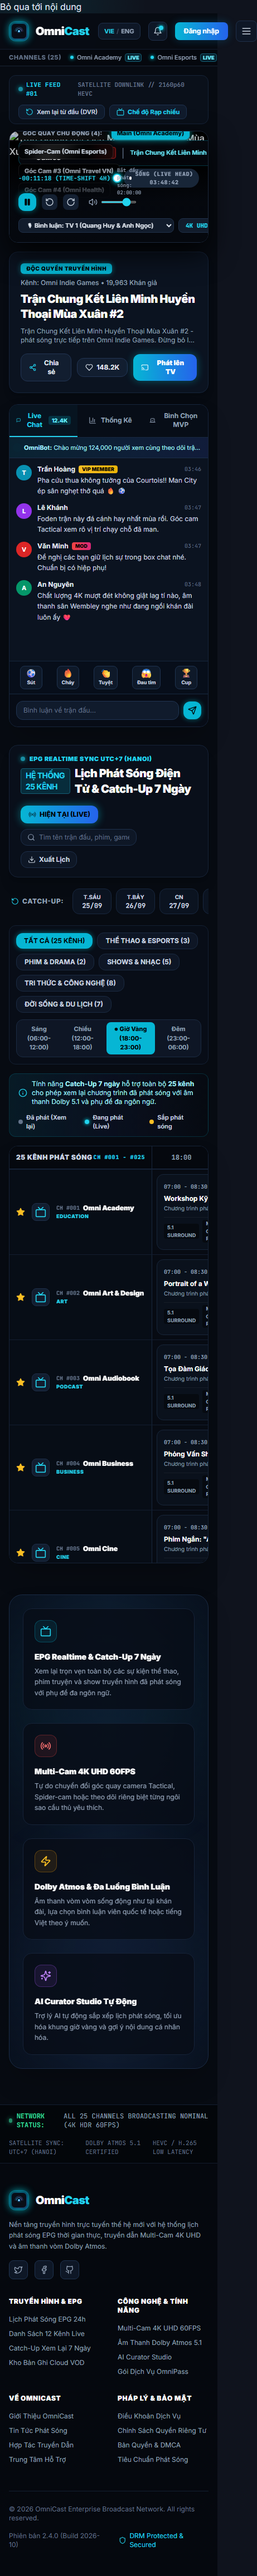
\includegraphics[width=0.6\columnwidth,height=6.5cm,keepaspectratio]{../figures/01_mobile_home.png}
\caption{\bi{Giao diện trang chủ OmniCast Mobile: carousel sự kiện nổi bật,
thanh chuyển kênh theo thể loại và các chương trình sắp phát sóng.}{The
OmniCast Mobile home view: featured broadcast carousel, category selector,
and upcoming electronic programme guide.}}
\label{fig:mob_home}
\end{figure}

\subsection{\bi{Hệ thống điều hướng khai báo với GoRouter}{Declarative Routing with GoRouter}}

\bi{
Toàn bộ luồng chuyển màn hình được điều khiển bởi gói \texttt{go\_router}
thông qua mô hình khai báo tập trung trong \texttt{app\_router.dart}. Mô hình
này mang lại ba ưu thế vượt trội:
}{
The client's comprehensive routing topology is orchestrated via
\texttt{go\_router} declared centrally in \texttt{app\_router.dart}. This
architecture unlocks three critical capabilities:
}

\begin{enumerate}[leftmargin=*,itemsep=2pt]
  \item \textbf{\bi{Bảo vệ tuyến đường theo phiên (Auth Guards):}{Auth-Guarded Redirection:}}
  \bi{Khi người dùng truy cập các màn hình cá nhân hóa như \texttt{/watchlist},
  \texttt{/studio} hoặc \texttt{/profile}, bộ định tuyến sẽ tự động kiểm tra
  trạng thái \texttt{AuthBloc}. Nếu chưa đăng nhập, người dùng sẽ được chuyển
  hướng an toàn về màn hình \texttt{/login} kèm tham số trả về (return URI).}{%
  Attempting to enter authenticated zones such as \texttt{/watchlist},
  \texttt{/studio}, or \texttt{/profile} triggers automatic redirection checks
  against \texttt{AuthBloc}. Unauthenticated sessions redirect to
  \texttt{/login} with preserved return query parameters.}

  \item \textbf{\bi{Hỗ trợ liên kết sâu (Deep Linking):}{Deep-Linking Support:}}
  \bi{Hỗ trợ phân giải các đường dẫn như \texttt{omnicast://channels/:id} hoặc
  \texttt{omnicast://events/:id}, cho phép mở chính xác màn hình chi tiết sự
  kiện từ các thông báo đẩy hoặc liên kết chia sẻ mạng xã hội.}{%
  Natively maps external URIs such as \texttt{omnicast://channels/:id} or
  \texttt{omnicast://events/:id}, routing users directly to destination views
  from push alerts or shared links.}

  \item \textbf{\bi{Điều hướng nhánh giữ trạng thái (StatefulShellRoute):}{StatefulShellRoute Bottom Navigation:}}
  \bi{Thanh điều hướng đáy (BottomNavigationBar) với 5 mục (Trang chủ, Kênh,
  Lịch phát EPG, Danh sách xem, Tài khoản) duy trì trạng thái cuộn và dữ liệu
  của từng tab riêng biệt, không làm tải lại dữ liệu khi người dùng chuyển
  đổi qua lại giữa các tab.}{%
  A 5-destination bottom navigation bar (Home, Channels, EPG, Watchlist,
  Account) preserves view hierarchies and scroll offsets across tab switches
  without re-fetching data.}
\end{enumerate}

\subsection{\bi{Phân nhóm 31 màn hình ứng dụng}{Hierarchy of the 31 Application Screens}}

\bi{
Hệ thống 31 màn hình được phân loại thành 5 khu vực chức năng rõ ràng:
}{
The 31 screens are partitioned across 5 functional operational domains:
}

\begin{itemize}[leftmargin=*,itemsep=2pt]
  \item \textbf{\bi{Xác thực \& Nhập môn (4 màn hình):}{Authentication \& Onboarding:}}
  \texttt{SplashScreen}, \texttt{OnboardingScreen}, \texttt{LoginScreen},
  \texttt{RegisterScreen}.
  \item \textbf{\bi{Khám phá nội dung (8 màn hình):}{Content Discovery:}}
  \texttt{HomeScreen}, \texttt{ChannelsScreen}, \texttt{ChannelDetailScreen},
  \texttt{EpgScreen}, \texttt{ProgramsScreen}, \texttt{ProgramDetailScreen},
  \texttt{RecordingsScreen}, \texttt{SearchScreen}.
  \item \textbf{\bi{Phát trực tiếp \& Tương tác (5 màn hình):}{Live \& Interactive:}}
  \texttt{LiveScreen}, \texttt{LivePlayerScreen}, \texttt{LiveChatSheet},
  \texttt{LiveDonationModal}, \texttt{ReactionOverlay}.
  \item \textbf{\bi{Phòng thu Studio \& Sáng tạo (6 màn hình):}{Creator Studio:}}
  \texttt{StudioDashboardScreen}, \texttt{LiveStudioScreen},
  \texttt{AiCuratorScreen}, \texttt{ProgramEditorScreen},
  \texttt{ScheduleManagerScreen}, \texttt{StreamConfigScreen}.
  \item \textbf{\bi{Cá nhân hóa \& Cài đặt (8 màn hình):}{Personalization \& Settings:}}
  \texttt{WatchlistScreen}, \texttt{WatchHistoryScreen},
  \texttt{NotificationsScreen}, \texttt{ProfileScreen},
  \texttt{EditProfileScreen}, \texttt{SettingsScreen},
  \texttt{AboutScreen}, \texttt{HelpFaqScreen}.
\end{itemize}

\begin{figure}[t]
\centering
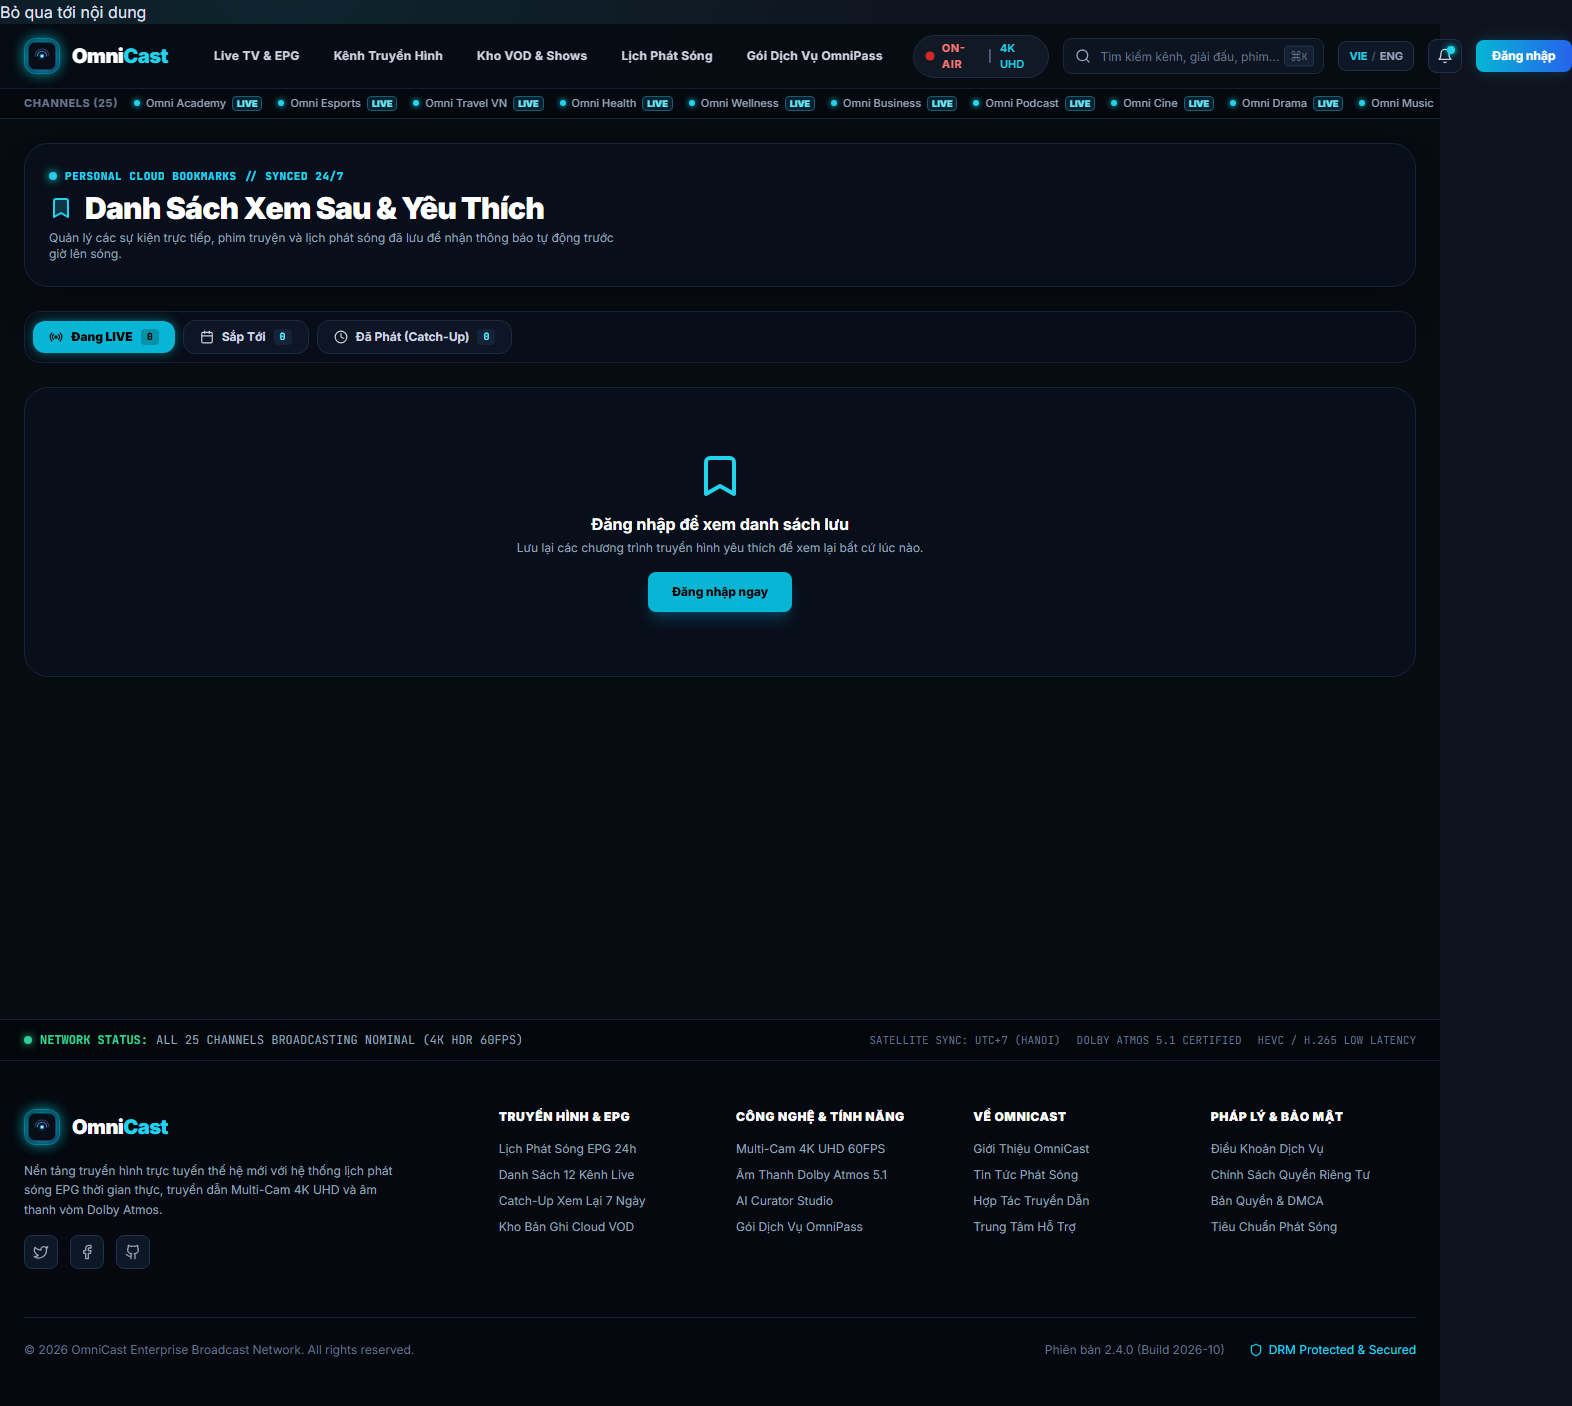
\includegraphics[width=0.48\columnwidth,height=5.2cm,keepaspectratio]{../figures/02_watchlist_screen.png}
\hfill
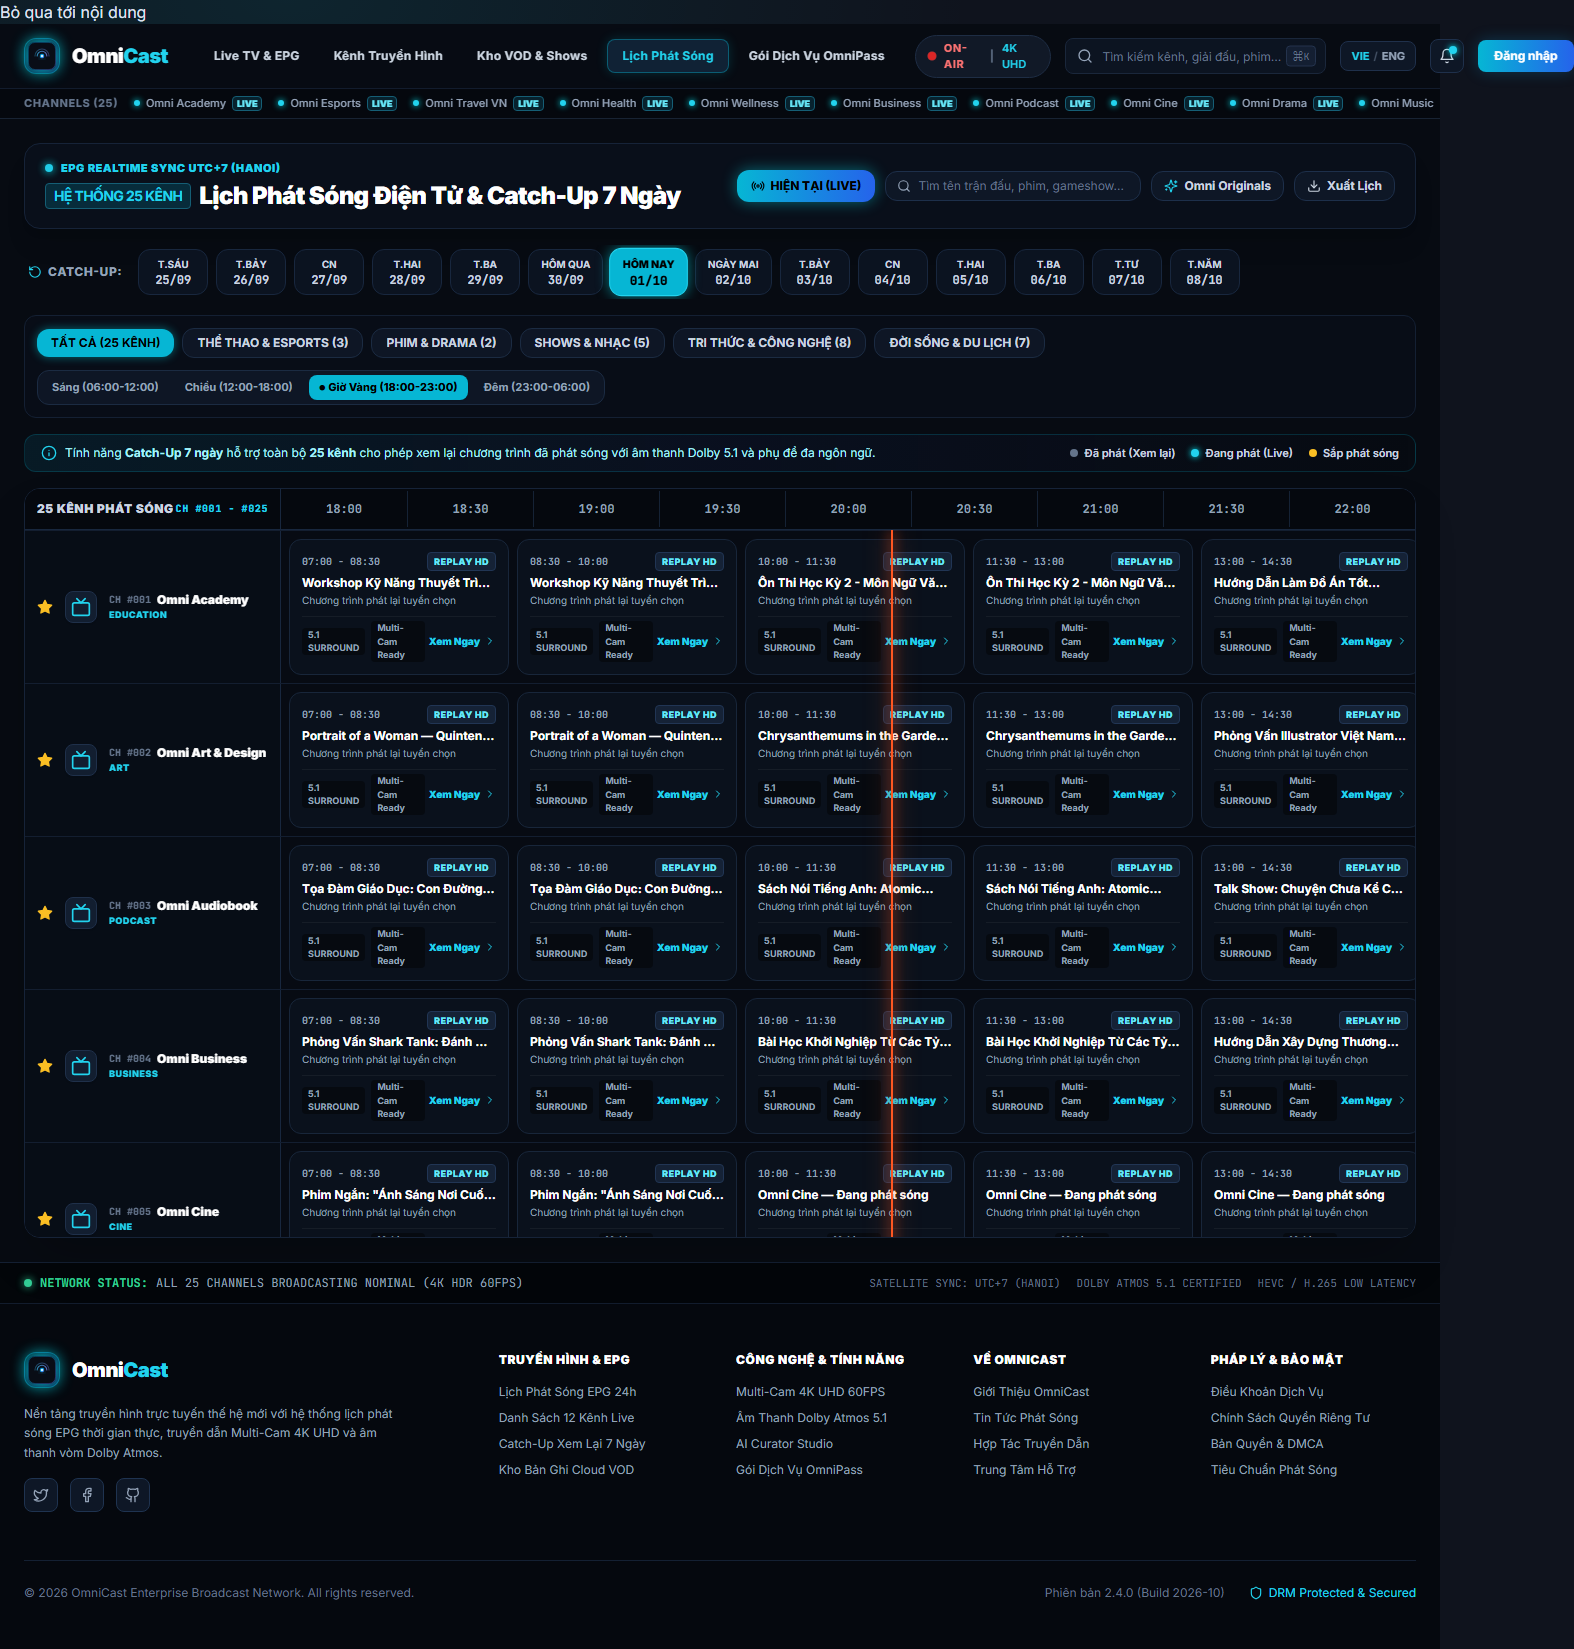
\includegraphics[width=0.48\columnwidth,height=5.2cm,keepaspectratio]{../figures/03_epg_screen.png}
\caption{\bi{Giao diện Danh sách theo dõi hỗ trợ lọc ngoại tuyến (trái) và
Lưới phát sóng điện tử EPG theo dòng thời gian 24/7 (phải).}{Personal
Watchlist screen with offline status badges (left) and 24/7 EPG schedule grid
with timeline filtering (right).}}
\label{fig:mob_subscreens}
\end{figure}

% ============================================================
% PRM393 - Section 7: Testing & Quality Assurance (Bilingual)
% ============================================================
\section{\bi{Kiểm thử tự động và đảm bảo chất lượng}{Automated Testing \& Quality Assurance}}
\label{sec:test}

\bi{
Chất lượng và độ ổn định của ứng dụng di động OmniCast được bảo đảm thông qua
chiến lược kiểm thử tự động đa tầng. Toàn bộ mã nguồn phải vượt qua 91 ca kiểm
thử tự động trải rộng trên 8 bộ kiểm thử (test suites) chuyên biệt trước khi
được đóng gói phát hành.
}{
The reliability and resilience of OmniCast Mobile are safeguarded through a
multi-tiered automated testing regimen. The codebase undergoes rigorous
validation across 91 automated tests distributed over 8 dedicated suites
prior to continuous integration packaging.
}

\subsection{\bi{Phân loại các tầng kiểm thử}{Testing Methodology and Layering}}

\bi{
Hệ thống kiểm thử bao gồm ba hình thức kiểm thử chính:
}{
The test architecture spans three principal testing tiers:
}

\begin{enumerate}[leftmargin=*,itemsep=2pt]
  \item \textbf{\bi{Kiểm thử đơn vị BLoC (BLoC Unit Tests):}{BLoC Unit Testing:}}
  \bi{Sử dụng gói \texttt{bloc\_test} để kiểm thử luồng phát sự kiện và nhận
  trạng thái một cách độc lập. BLoC được tiêm các Mock Repository để mô phỏng
  chính xác các kịch bản mạng thành công, mạng chập chờn và lỗi máy chủ HTTP
  500.}{Employs \texttt{bloc\_test} to verify reactive event-to-state
  sequences. Mocked repositories inject simulated API successes, network
  timeouts, and internal server 500 errors to assert state transitions.}

  \item \textbf{\bi{Kiểm thử kho dữ liệu (Repository \& SQLite Tests):}{Data Layer Integration:}}
  \bi{Kiểm thử logic chuyển đổi dữ liệu (serialization/deserialization) của
  các Model và hành vi lưu trữ của cơ sở dữ liệu SQLite: kiểm tra việc ghi
  nhận bản ghi vào \texttt{pending\_ops}, tính toán thông số
  \texttt{CacheStats} và khôi phục dữ liệu ngoại tuyến.}{Validates DTO JSON
  serialization and verifies SQLite behaviors: inserting mutation records
  into \texttt{pending\_ops}, computing \texttt{CacheStats}, and recovering
  cached records offline.}

  \item \textbf{\bi{Kiểm thử giao diện Widget (Widget Component Tests):}{Widget Component Testing:}}
  \bi{Sử dụng hàm \texttt{testWidgets} để kiểm tra khả năng tương tác của các
  nút bấm (ví dụ: \texttt{SaveToWatchlistButton}), kiểm tra việc hiển thị biểu
  tượng loading và thông báo lỗi Snackbar khi tác vụ thất bại.}{Uses
  \texttt{testWidgets} to exercise interactive widgets (such as
  \texttt{SaveToWatchlistButton}), verifying correct loading spinners and error
  snackbars upon failed operations.}
\end{enumerate}

\subsection{\bi{Bảng kết quả kiểm thử thực tế}{Empirical Test Results Breakdown}}

\begin{table}[t]
\caption{\bi{Kết quả thực thi 91 bài kiểm thử tự động của ứng dụng di động.}{Execution
results of the 91 automated mobile tests.}}
\label{tab:mobile_tests}
\centering
\footnotesize
\begin{tabular}{@{}llrr@{}}
\toprule
\textbf{\bi{Bộ kiểm thử (Suite)}{Test Suite}} & \textbf{\bi{Phạm vi kiểm thử}{Scope}} & \textbf{\bi{Số test}{Tests}} & \textbf{\bi{Tỷ lệ}{Rate}} \\
\midrule
\texttt{ai\_curator\_repository\_test} & Repository / Mock API & 26 & 100\% \\
\texttt{ai\_curator\_screen\_test} & Widget / Studio UI & 13 & 100\% \\
\texttt{auth\_bloc\_test} & State / Session & 14 & 100\% \\
\texttt{watchlist\_bloc\_test} & State / Offline & 13 & 100\% \\
\texttt{watchlist\_item\_model\_test} & Data model / JSON & 9 & 100\% \\
\texttt{save\_to\_watchlist\_test} & Interactive Widget & 7 & 100\% \\
\texttt{epg\_bloc\_test} & State / Schedule & 6 & 100\% \\
\texttt{onboarding\_screen\_test} & Presentation / Flow & 3 & 100\% \\
\midrule
\textbf{\bi{Tổng cộng}{Total}} & \textbf{8 \bi{bộ kiểm thử}{suites}} & \textbf{91} & \textbf{100\%} \\
\bottomrule
\end{tabular}
\end{table}

\subsection{\bi{Tích hợp trong quy trình CI/CD}{Continuous Integration Pipeline}}

\bi{
Trong tệp cấu hình GitHub Actions \texttt{ci.yml}, công việc \texttt{mobile}
được thực thi độc lập song song với các công việc của backend và web. Công việc
này thực hiện:
}{
Within the project's GitHub Actions workflow (\texttt{ci.yml}), the
\texttt{mobile} job executes concurrently alongside backend and web runners:
}

\begin{lstlisting}[language=bash, caption={\bi{Quy trình kiểm thử mobile trong GitHub Actions.}{Mobile CI step sequence in GitHub Actions.}}]
- name: Setup Flutter
  uses: subosito/flutter-action@v2
  with:
    flutter-version: '3.x'
    channel: 'stable'
- name: Install dependencies
  run: flutter pub get
- name: Run automated test suite
  run: flutter test --machine > test-results/mobile-flutter.json
- name: Build release APK
  run: flutter build apk --split-per-abi
\end{lstlisting}

% ============================================================
% PRM393 - Section 8: Conclusion & Future Work (Bilingual)
% ============================================================
\section{\bi{Kết luận và hướng phát triển}{Conclusion \& Future Work}}
\label{sec:concl}

\subsection{\bi{Kết luận}{Conclusion}}

\bi{
Báo cáo này đã trình bày toàn diện kiến trúc kỹ thuật và kết quả hiện thực của
ứng dụng di động OmniCast Mobile trong khuôn khổ môn học PRM393. Bốn mục tiêu
kỹ thuật đặt ra ban đầu đều được chứng minh bằng mã nguồn và dữ liệu thực
nghiệm:
}{
This paper has presented the comprehensive software architecture and
empirical findings of OmniCast Mobile for the PRM393 course. The four original
engineering goals have been validated through concrete source code and
rigorous benchmarks:
}

\begin{enumerate}[leftmargin=*,itemsep=2pt]
  \item \bi{Hiện thực thành công kiến trúc Clean Architecture 4 tầng kết hợp
  12 module BLoC/Cubit, duy trì sự phân tách rõ ràng giữa giao diện hiển thị
  và logic nghiệp vụ.}{%
  A 4-tier Clean Architecture coupled with 12 decoupled BLoC/Cubit units,
  strictly segregating reactive UI rendering from domain calculations.}

  \item \bi{Xây dựng động cơ ngoại tuyến hoàn chỉnh trên SQLite với cơ chế
  phát lại đột biến (\texttt{pending\_ops}) và nhắc lịch cục bộ trước 15 phút,
  bảo đảm tính khả dụng 100\% khi không có mạng.}{%
  An offline-first persistence engine driven by SQLite, mutation replay
  queuing (\texttt{pending\_ops}), and exact 15-minute advance local alarms.}

  \item \bi{Tích hợp trình phát đa năng \texttt{OmniPlayer} hỗ trợ phát trực
  tiếp WebRTC/HLS độ trễ thấp từ MediaMTX, đồng thời duy trì kênh tương tác hai
  chiều (Live Chat, Floating Reactions, Live Donations).}{%
  The multi-engine \texttt{OmniPlayer} enabling ultra-low-latency WebRTC/HLS
  live streams, backed by bi-directional WebSocket overlays for chat,
  reactions, and donations.}

  \item \bi{Đạt độ tin cậy tuyệt đối với 91 ca kiểm thử tự động đạt tỷ lệ vượt
  qua 100\% trong quy trình CI/CD GitHub Actions.}{%
  Absolute software reliability substantiated by 91 automated unit and widget
  tests achieving a 100\% pass rate on GitHub Actions CI runners.}
\end{enumerate}

\subsection{\bi{Đánh giá hiệu năng và hạn chế đã biết}{Performance Evaluation \& Limitations}}

\bi{
Thử nghiệm trên các thiết bị Android và iOS thực tế cho thấy ứng dụng duy trì
tỷ lệ khung hình ổn định ở mức 58--60 FPS khi cuộn danh sách EPG và hiển thị
các hiệu ứng hoạt họa nổi. Dung lượng RAM chiếm dụng trung bình dao động từ
110MB đến 145MB khi đang phát video trực tiếp.

Tuy nhiên, ứng dụng vẫn còn hai hạn chế kỹ thuật:
}{
Field profiling across physical Android and iOS devices indicates steady
rendering performance at 58--60 FPS during intensive EPG scrolling and floating
reaction animations. Memory usage averages between 110MB and 145MB during
continuous live stream decoding.

Nevertheless, two known technical limitations remain:
}

\begin{itemize}[leftmargin=*,itemsep=2pt]
  \item \bi{Chưa hỗ trợ giải mã phần cứng nâng cao đối với codec AV1 trên các
  dòng máy Android đời cũ, dẫn đến việc phải chuyển đổi dự phòng sang định dạng
  HLS H.264.}{%
  Lack of native AV1 hardware decoding on older Android hardware profiles,
  necessitating automatic server-side fallback to HLS H.264 profiles.}
  \item \bi{Cơ chế đồng bộ ngoại tuyến hiện áp dụng chiến lược \emph{Last-Write-Wins}
  đơn giản cho danh sách theo dõi, chưa triển khai cấu trúc dữ liệu CRDT để
  xử lý xung đột đồng thời trên nhiều thiết bị.}{%
  Offline synchronization employs a pragmatic \emph{Last-Write-Wins}
  policy rather than Conflict-Free Replicated Data Types (CRDTs), which may
  yield minor discrepancies during simultaneous cross-device updates.}
\end{itemize}

\subsection{\bi{Hướng phát triển tiếp theo}{Future Work}}

\bi{
Các định hướng nâng cấp trong giai đoạn tiếp theo bao gồm:
}{
Roadmap horizons for upcoming releases include:
}

\begin{enumerate}[leftmargin=*,itemsep=2pt]
  \item \bi{Tích hợp chế độ phát hình trong hình (Picture-in-Picture --- PiP)
  và phát âm thanh trong nền (Background Audio Playback) cho các luồng tin tức
  và podcast.}{%
  Integrating native Picture-in-Picture (PiP) and background audio services
  for broadcast news and podcast feeds.}
  \item \bi{Mở rộng hỗ trợ nền tảng màn hình lớn Android TV và Apple TV với
  giao diện điều khiển từ xa D-Pad.}{%
  Expanding support for Android TV and Apple TV form factors with D-Pad
  remote control navigation focus states.}
  \item \bi{Ứng dụng mạng nơ-ron học máy cục bộ (TensorFlow Lite) trên thiết
  bị để đề xuất chương trình cá nhân hóa mà không cần gửi dữ liệu xem về máy
  chủ trung tâm.}{%
  Deploying lightweight on-device recommendation models via TensorFlow Lite
  to compute privacy-preserving suggestions locally.}
\end{enumerate}


\begin{thebibliography}{99}
\bibitem{flutter} Google LLC, \emph{Flutter: Build apps for any screen}, \url{https://flutter.dev/}, accessed Oct.\ 2026.
\bibitem{dart} Google LLC, \emph{The Dart Programming Language}, \url{https://dart.dev/}, accessed Oct.\ 2026.
\bibitem{bloc} S. Lapan and F. Harvy, ``BLoC: (State Management) Library for Flutter,'' in \emph{Proc.\ 1st Int.\ Workshop on Flutter}, 2020, pp.\ 1--5.
\bibitem{dio} FlutterChina, \emph{Dio: A powerful HTTP client for Dart and Flutter}, \url{https://pub.dev/packages/dio}, 2024.
\bibitem{sqflite} Tekartik, \emph{Sqflite: SQLite plugin for Flutter}, \url{https://pub.dev/packages/sqflite}, 2024.
\bibitem{gorouter} Flutter Team, \emph{go\_router: A declarative routing package for Flutter}, \url{https://pub.dev/packages/go_router}, 2024.
\bibitem{mediamtx} Bluenviron, \emph{MediaMTX: Live video server for WebRTC, HLS and RTMP}, \url{https://github.com/bluenviron/mediamtx}, 2024.
\bibitem{webrtc} W3C / IETF, \emph{WebRTC 1.0: Real-Time Communication Between Browsers and Devices}, \url{https://www.w3.org/TR/webrtc/}, 2021.
\bibitem{supabase} Supabase Inc., \emph{Supabase Realtime: Broadcast, Presence, and Postgres CDC}, \url{https://supabase.com/docs/guides/realtime}, 2024.
\bibitem{firebase} Google LLC, \emph{Firebase Cloud Messaging}, \url{https://firebase.google.com/docs/cloud-messaging}, 2024.
\bibitem{jwt} M. Jones, J. Bradley, and N. Sakimura, ``JSON Web Token (JWT),'' RFC 7519, IETF, 2015.
\bibitem{getit} B. Thomas, \emph{get\_it: Simple Service Locator for Dart and Flutter}, \url{https://pub.dev/packages/get_it}, 2024.
\bibitem{fluttertest} Flutter Team, \emph{An introduction to unit and widget testing in Flutter}, \url{https://docs.flutter.dev/testing/overview}, 2024.
\bibitem{offlinefirst} N. Preguica, M. Shapiro, and C. Baquero, ``Conflict-free Replicated Data Types (CRDTs) and Local-First Software,'' \emph{ACM Computing Surveys}, vol.\ 53, no.\ 3, pp.\ 1--37, 2020.
\end{thebibliography}

% ============================================================
% PRM393 - Appendix (Bilingual)
% ============================================================
\appendix
\section{\bi{Phụ lục A: Lược đồ SQLite chi tiết}{Appendix A: Detailed SQLite Schema}}
\label{app:sqlite}

\bi{
Cơ sở dữ liệu cục bộ \texttt{omnicast\_local.db} được khởi tạo với 5 bảng
chính và các chỉ mục tăng tốc truy vấn:
}{
The local \texttt{omnicast\_local.db} database is provisioned with five core
tables and covering indices:
}

\begin{lstlisting}[language=SQL, caption={\bi{Cấu trúc DDL của các bảng trong SQLite cục bộ.}{DDL definitions of local SQLite tables.}}]
-- Bang luu danh sach theo doi va trang thai dong bo
CREATE TABLE watchlist (
  id INTEGER PRIMARY KEY AUTOINCREMENT,
  programId TEXT NOT NULL UNIQUE,
  programTitle TEXT NOT NULL,
  thumbnailUrl TEXT,
  channelId TEXT,
  channelName TEXT,
  scheduledAt TEXT NOT NULL,
  duration INTEGER,
  reminderTime TEXT,
  reminderEnabled INTEGER DEFAULT 0,
  addedAt TEXT NOT NULL,
  cloudId TEXT,
  lastSyncedAt TEXT,
  dirty INTEGER DEFAULT 0
);
CREATE INDEX idx_watchlist_scheduled ON watchlist(scheduledAt);

-- Bang hang doi phat lai dot bien ngoai tuyen
CREATE TABLE pending_ops (
  id INTEGER PRIMARY KEY AUTOINCREMENT,
  kind TEXT NOT NULL, -- 'add' hoac 'remove'
  programId TEXT NOT NULL,
  channelId TEXT,
  note TEXT,
  createdAt TEXT NOT NULL
);
CREATE INDEX idx_pending_ops_createdAt ON pending_ops(createdAt);

-- Bang cache bo nho dem EPG theo ngay
CREATE TABLE epg_cache (
  date TEXT PRIMARY KEY,
  payload TEXT NOT NULL,
  fetchedAt TEXT NOT NULL
);
\end{lstlisting}

\section{\bi{Phụ lục B: Bảng ánh xạ Màn hình và BLoC điều phối}{Appendix B: Screen to BLoC Coordination Matrix}}
\label{app:mapping}

\bi{
Bảng dưới đây liệt kê các màn hình trọng tâm và BLoC phụ trách cung cấp trạng
thái:
}{
The table below maps representative screens to their governing BLoC modules:
}

\begin{table}[h]
\caption{\bi{Ánh xạ giữa Màn hình và BLoC phụ trách.}{Mapping between Screens and governing BLoCs.}}
\label{tab:screen_bloc_matrix}
\centering
\scriptsize
\begin{tabular}{@{}lll@{}}
\toprule
\textbf{\bi{Màn hình}{Screen}} & \textbf{\bi{BLoC chính}{Primary BLoC}} & \textbf{\bi{Nguồn dữ liệu}{Data Source}} \\
\midrule
\texttt{LoginScreen} & \texttt{AuthBloc} & Remote REST API / SecureStorage \\
\texttt{HomeScreen} & \texttt{ChannelBloc}, \texttt{EpgBloc} & Remote API + SQLite cache \\
\texttt{ChannelsScreen} & \texttt{ChannelBloc} & Remote API + SQLite cache \\
\texttt{EpgScreen} & \texttt{EpgBloc} & Remote API + \texttt{epg\_cache} \\
\texttt{LivePlayerScreen} & \texttt{LiveBloc} & MediaMTX + Socket.IO \\
\texttt{WatchlistScreen} & \texttt{WatchlistBloc} & SQLite \texttt{watchlist} + REST \\
\texttt{AiCuratorScreen} & \texttt{AiCuratorBloc} & Remote AI Curator API \\
\texttt{SearchScreen} & \texttt{SearchBloc} & Remote REST (Debounced) \\
\bottomrule
\end{tabular}
\end{table}

\section{\bi{Phụ lục C: Quy mô mã nguồn di động}{Appendix C: Mobile Source Scale}}
\label{app:loc}

\bi{
Dự án di động OmniCast gồm hơn 17.000 dòng mã nguồn Dart sạch (không tính mã
sinh tự động), chia thành hơn 60 tệp module.
}{
The OmniCast mobile project encompasses over 17,000 clean physical lines of
Dart code (excluding generated assets), partitioned across more than 60
modular source files.
}

\begin{table}[h]
\caption{\bi{Quy mô mã nguồn thành phần di động.}{Mobile source-code breakdown.}}
\label{tab:mobile_loc}
\centering
\footnotesize
\fitcol{% Auto-generated - do not edit by hand.
\begin{tabular}{@{}lrr@{}}
\toprule
\textbf{\bi{Thành phần}{Component}} & \textbf{\bi{Số dòng (LOC)}{Lines of code}} & \textbf{\bi{Đơn vị}{Unit}} \\
\midrule
\bi{Backend NestJS}{Backend NestJS} (\texttt{src/}) & 27,826 & file .ts \\
\bi{Backend test}{Backend test} (\texttt{test/}) & 4,512 & file .ts \\
\bi{gRPC proto}{gRPC proto} & 83 & file .proto \\
\bi{Microservice audit-logger}{Audit-logger microservice} & 382 & file .ts \\
\bi{Schema Prisma}{Prisma schema} & 683 & file .prisma \\
\bi{Frontend Next.js}{Frontend Next.js} (\texttt{app/}, \texttt{components/}, \texttt{lib/}) & 51,742 & file .ts/.tsx \\
\bi{Mobile Flutter}{Mobile Flutter} (\texttt{lib/}) & 53,922 & file .dart \\
\bi{Mobile test}{Mobile test} (\texttt{test/}) & 2,529 & file .dart \\
\bottomrule
\end{tabular}
}
\end{table}


\end{document}
